\documentclass[]{article}
\usepackage{lmodern}
\usepackage{amssymb,amsmath}
\usepackage{ifxetex,ifluatex}
\usepackage{fixltx2e} % provides \textsubscript
\ifnum 0\ifxetex 1\fi\ifluatex 1\fi=0 % if pdftex
  \usepackage[T1]{fontenc}
  \usepackage[utf8]{inputenc}
\else % if luatex or xelatex
  \ifxetex
    \usepackage{mathspec}
  \else
    \usepackage{fontspec}
  \fi
  \defaultfontfeatures{Ligatures=TeX,Scale=MatchLowercase}
\fi
% use upquote if available, for straight quotes in verbatim environments
\IfFileExists{upquote.sty}{\usepackage{upquote}}{}
% use microtype if available
\IfFileExists{microtype.sty}{%
\usepackage[]{microtype}
\UseMicrotypeSet[protrusion]{basicmath} % disable protrusion for tt fonts
}{}
\PassOptionsToPackage{hyphens}{url} % url is loaded by hyperref
\usepackage[unicode=true]{hyperref}
\hypersetup{
            pdfborder={0 0 0},
            breaklinks=true}
\urlstyle{same}  % don't use monospace font for urls
\usepackage{color}
\usepackage{fancyvrb}
\newcommand{\VerbBar}{|}
\newcommand{\VERB}{\Verb[commandchars=\\\{\}]}
\DefineVerbatimEnvironment{Highlighting}{Verbatim}{commandchars=\\\{\}}
% Add ',fontsize=\small' for more characters per line
\newenvironment{Shaded}{}{}
\newcommand{\KeywordTok}[1]{\textcolor[rgb]{0.00,0.44,0.13}{\textbf{#1}}}
\newcommand{\DataTypeTok}[1]{\textcolor[rgb]{0.56,0.13,0.00}{#1}}
\newcommand{\DecValTok}[1]{\textcolor[rgb]{0.25,0.63,0.44}{#1}}
\newcommand{\BaseNTok}[1]{\textcolor[rgb]{0.25,0.63,0.44}{#1}}
\newcommand{\FloatTok}[1]{\textcolor[rgb]{0.25,0.63,0.44}{#1}}
\newcommand{\ConstantTok}[1]{\textcolor[rgb]{0.53,0.00,0.00}{#1}}
\newcommand{\CharTok}[1]{\textcolor[rgb]{0.25,0.44,0.63}{#1}}
\newcommand{\SpecialCharTok}[1]{\textcolor[rgb]{0.25,0.44,0.63}{#1}}
\newcommand{\StringTok}[1]{\textcolor[rgb]{0.25,0.44,0.63}{#1}}
\newcommand{\VerbatimStringTok}[1]{\textcolor[rgb]{0.25,0.44,0.63}{#1}}
\newcommand{\SpecialStringTok}[1]{\textcolor[rgb]{0.73,0.40,0.53}{#1}}
\newcommand{\ImportTok}[1]{#1}
\newcommand{\CommentTok}[1]{\textcolor[rgb]{0.38,0.63,0.69}{\textit{#1}}}
\newcommand{\DocumentationTok}[1]{\textcolor[rgb]{0.73,0.13,0.13}{\textit{#1}}}
\newcommand{\AnnotationTok}[1]{\textcolor[rgb]{0.38,0.63,0.69}{\textbf{\textit{#1}}}}
\newcommand{\CommentVarTok}[1]{\textcolor[rgb]{0.38,0.63,0.69}{\textbf{\textit{#1}}}}
\newcommand{\OtherTok}[1]{\textcolor[rgb]{0.00,0.44,0.13}{#1}}
\newcommand{\FunctionTok}[1]{\textcolor[rgb]{0.02,0.16,0.49}{#1}}
\newcommand{\VariableTok}[1]{\textcolor[rgb]{0.10,0.09,0.49}{#1}}
\newcommand{\ControlFlowTok}[1]{\textcolor[rgb]{0.00,0.44,0.13}{\textbf{#1}}}
\newcommand{\OperatorTok}[1]{\textcolor[rgb]{0.40,0.40,0.40}{#1}}
\newcommand{\BuiltInTok}[1]{#1}
\newcommand{\ExtensionTok}[1]{#1}
\newcommand{\PreprocessorTok}[1]{\textcolor[rgb]{0.74,0.48,0.00}{#1}}
\newcommand{\AttributeTok}[1]{\textcolor[rgb]{0.49,0.56,0.16}{#1}}
\newcommand{\RegionMarkerTok}[1]{#1}
\newcommand{\InformationTok}[1]{\textcolor[rgb]{0.38,0.63,0.69}{\textbf{\textit{#1}}}}
\newcommand{\WarningTok}[1]{\textcolor[rgb]{0.38,0.63,0.69}{\textbf{\textit{#1}}}}
\newcommand{\AlertTok}[1]{\textcolor[rgb]{1.00,0.00,0.00}{\textbf{#1}}}
\newcommand{\ErrorTok}[1]{\textcolor[rgb]{1.00,0.00,0.00}{\textbf{#1}}}
\newcommand{\NormalTok}[1]{#1}
\usepackage{graphicx,grffile}
\makeatletter
\def\maxwidth{\ifdim\Gin@nat@width>\linewidth\linewidth\else\Gin@nat@width\fi}
\def\maxheight{\ifdim\Gin@nat@height>\textheight\textheight\else\Gin@nat@height\fi}
\makeatother
% Scale images if necessary, so that they will not overflow the page
% margins by default, and it is still possible to overwrite the defaults
% using explicit options in \includegraphics[width, height, ...]{}
\setkeys{Gin}{width=\maxwidth,height=\maxheight,keepaspectratio}
\IfFileExists{parskip.sty}{%
\usepackage{parskip}
}{% else
\setlength{\parindent}{0pt}
\setlength{\parskip}{6pt plus 2pt minus 1pt}
}
\setlength{\emergencystretch}{3em}  % prevent overfull lines
\providecommand{\tightlist}{%
  \setlength{\itemsep}{0pt}\setlength{\parskip}{0pt}}
\setcounter{secnumdepth}{0}
% Redefines (sub)paragraphs to behave more like sections
\ifx\paragraph\undefined\else
\let\oldparagraph\paragraph
\renewcommand{\paragraph}[1]{\oldparagraph{#1}\mbox{}}
\fi
\ifx\subparagraph\undefined\else
\let\oldsubparagraph\subparagraph
\renewcommand{\subparagraph}[1]{\oldsubparagraph{#1}\mbox{}}
\fi

% set default figure placement to htbp
\makeatletter
\def\fps@figure{htbp}
\makeatother


\date{}

%
% Tesi D.S.I. - modello preso da
% Stanford University PhD thesis style -- modifications to the report style
%
%%%%%%%%%%%%%%%%%%%%%%%%%%%%%%%%%%%%%%%%%%%%%%%%%%%%%%%%%%%%%%%%%%%%%%%%%%%
%                                                                         %
%			TESI DOTTORATO                                                   %
%			______________                                                   %
%                                                                         %
%			AUTORE: Elena Pagani                                             %
%                                                                         %
%			Ultima revisione: 7.X.1998                                       %
%                                                                         %
%%%%%%%%%%%%%%%%%%%%%%%%%%%%%%%%%%%%%%%%%%%%%%%%%%%%%%%%%%%%%%%%%%%%%%%%%%%
%
%
%    \renewcommand{\baselinestretch}{1.6}      % interline spacing
%
% \includeonly{}
%
%			PREAMBOLO
%
\usepackage{amssymb,amsmath,amsthm}
\usepackage{graphicx}
\usepackage{url}
\usepackage{hyperref}
\usepackage{epsfig}
\usepackage[italian]{babel}
\usepackage{tesi}

% per le accentate
\usepackage[utf8]{inputenc}
%
\newtheorem{myteor}{Teorema}[section]
%
\newenvironment{teor}{\begin{myteor}\sl}{\end{myteor}}
%
%
%			TITOLO
%
\begin{document}
\title{Kafka: streaming data}
\author{Stefano CARMIGNOLA}
\dept{Corso di Laurea in Informatica} 
\anno{2017-2018}
\matricola{21015}
\relatore{Prof. Alberto MOMIGLIANO}
\correlatore{Dr. Edmondo PORCU}
\beforepreface
\end{document}


 


\begin{document}

\section{Kafka: streaming data}\label{kafka-streaming-data}

\subsection{Indice}\label{indice}

\begin{enumerate}
\def\labelenumi{\arabic{enumi}.}
\tightlist
\item
  \protect\hyperlink{motivazioni}{Motivazioni}
\item
  \protect\hyperlink{introduzione}{Introduzione}
\item
  \protect\hyperlink{etl}{ETL}
\item
  \protect\hyperlink{event-sourcing}{Event sourcing}\\
  4.1. \protect\hyperlink{es-intro}{L'importanza dei dati e degli
  eventi}\\
  4.2. \protect\hyperlink{es-desc}{Descrizione}\\
  4.3. \protect\hyperlink{es-vantaggi}{Vantaggi}\\
  4.4. \protect\hyperlink{es-svantaggi}{Svantaggi}
\item
  \protect\hyperlink{kafka}{Apache Kafka: Ecosistema}\\
  5.1. \protect\hyperlink{kafka-intro}{Introduzione}\\
  5.2. \protect\hyperlink{kafka-msg}{Messaggi}\\
  5.3. \protect\hyperlink{kafka-topic}{Topic e partizioni}\\
  5.4. \protect\hyperlink{kafka-prod}{Producers}\\
  5.5. \protect\hyperlink{kafka-consum}{Consumers}\\
  5.6. \protect\hyperlink{kafka-brok}{Brokers e clusters}\\
  5.7. \protect\hyperlink{kafka-schm}{Schema}\\
  5.8. \protect\hyperlink{kafka-schm-re}{Schema registry}
\item
  \protect\hyperlink{architettura}{Architetture Event-driven}\\
  6.1. \protect\hyperlink{architettura-intro}{Kafka come piattaforma per
  Event Sourcing}\\
  6.2. \protect\hyperlink{architettura-conn}{Kafka Connect: sistemi
  legacy, database ed Event Sourcing}\\
  6.3. \protect\hyperlink{architettura-stream}{Kafka Streams}
\item
  \protect\hyperlink{conclusioni}{Conclusioni}
\item
  \protect\hyperlink{bibliografia}{Bibliografia}
\item
  \protect\hyperlink{sitografia}{Sitografia}
\end{enumerate}

\newpage

\hypertarget{motivazioni}{\subsection{1.
Motivazioni}\label{motivazioni}}

Negli ultimi anni l'avvento delle architetture a microservizi ha portato
la necessità di studiare nuove soluzioni al problema della gestione di
molteplici fonti di dati.

In sistemi complessi formati da più microservizi, svariati componenti
interdipendenti comunicano tra loro scambiandosi dati e attingendo da
numerose fonti di dati comuni come database, data warehouses oppure dei
servizi esterni.

La necessità di filtrare, standardizzare e gestire molte fonti di dati
aveva portato alla nascita del processo di \emph{Extract, Transform,
Load} (ETL) per l'estrazione, trasformazione e caricamento di dati in
sistemi di sintesi come data warehouse o data mart, questo processo si
sta però rivelando complicato, impegnativo e dispendioso in un mondo
dove la mole di dati prodotta dal logging di eventi critici per un
qualsiasi business è in continua crescita: semplici esempi sono la
gestione degli eventi in un sistema \emph{Internet of things} (IoT)
oppure lo studio delle abitudini dei propri clienti per un servizio
online.

Lo stream processing tra microservizi propone un nuovo approccio per la
gestione di questi problemi, fornendo una soluzione adatta alla gestione
di dati in real-time altamente scalabile e ad alto throughput.

Apache Kafka è una piattaforma di streaming dati nata in un contesto
aziendale importante che mira a rivoluzionare il modo con cui i
microservizi di un business comunicano tra loro, favorendo un approccio
improntato sulla gestione di eventi legati al comportamento dei dati,
più che i dati in se.\\
Kafka nasce per sfruttare a pieno lo stream processing e favorire una
gestione intelligente di grosse moli di dati, abbandonando il classico
processo ``batch'' ETL per una soluzione, appunto, basata sullo
streaming dei dati tra microservizi.

\newpage

\hypertarget{introduzione}{\subsection{2.
Introduzione}\label{introduzione}}

Prima di poter discutere della soluzione architetturale fornita da
Apache Kafka e quali vantaggi propone rispetto alle soluzioni di batch
ETL, è necessario approfondire alcuni temi tra cui il più importante è
sicurante event sourcing (ES).

Il terzo capitolo presenta una veloce descrizione di un processo ETL in
modo da dare visione del pattern strutturale per il quale si vuole dare
una alternativa con Kafka.

Il quarto capitolo è utilizzato per illustrare uno dei concetti chiave
della tesi: l'importanza di gestire e vedere le basi di dati come
eventi, perchè utilizzare il concetto di eventi per modelizzare i dati
ed infine, come utilizzare event sourcing.

Il quinto ed il sesto capitolo sono dedicati ad esaminare la piattaforma
Apache Kafka, sia da un punto di vista tecnico-architetturale
esaminandone le singole parti che compongono la piattaforma, sia
l'ecosistema che si è venuto a creare intorno alla piattaforma,
principalmente l'utilizzo delle librerie Kafka Connect e Kafka Streams;
Viene inoltre presentato come utilizzare ES nel contesto dell'uso della
piattaforma Kafka.

Infine nelle conclusioni vengono messi a confronto i processi ETL e la
soluzione di streaming di dati offerta da Kafka nel contesto della
gestione di grosse moli di dati tra microservizi e dei sistemi
distribuiti.

\newpage

\hypertarget{etl}{\subsection{3. ETL}\label{etl}}

Un processo di \emph{Extract, Transform, Load} (ETL) è un processo
mirato alla trasformazione di dati contenuti su più database per
ottenere un nuovo insieme di dati, filtrato e trasformato secondo una
particolare logica, destinato ad essere salvato in una data warehouse.

Verso la fine degli anni '70 molte aziende iniziarono ad utilizzare
molteplici database per salvare e gestire informazioni, è proprio in
questo contesto che nascono i processi di ETL: con l'avanzare del tempo
è stato necessario studiare un metodo per l'aggregazione e gestione
delle varie fonti di dati in modo tale da ottenere un insieme omogeno di
dati da utilizzare per operazioni di analisi o verifica relative al
business dell'azienda.

\begin{figure}
\centering
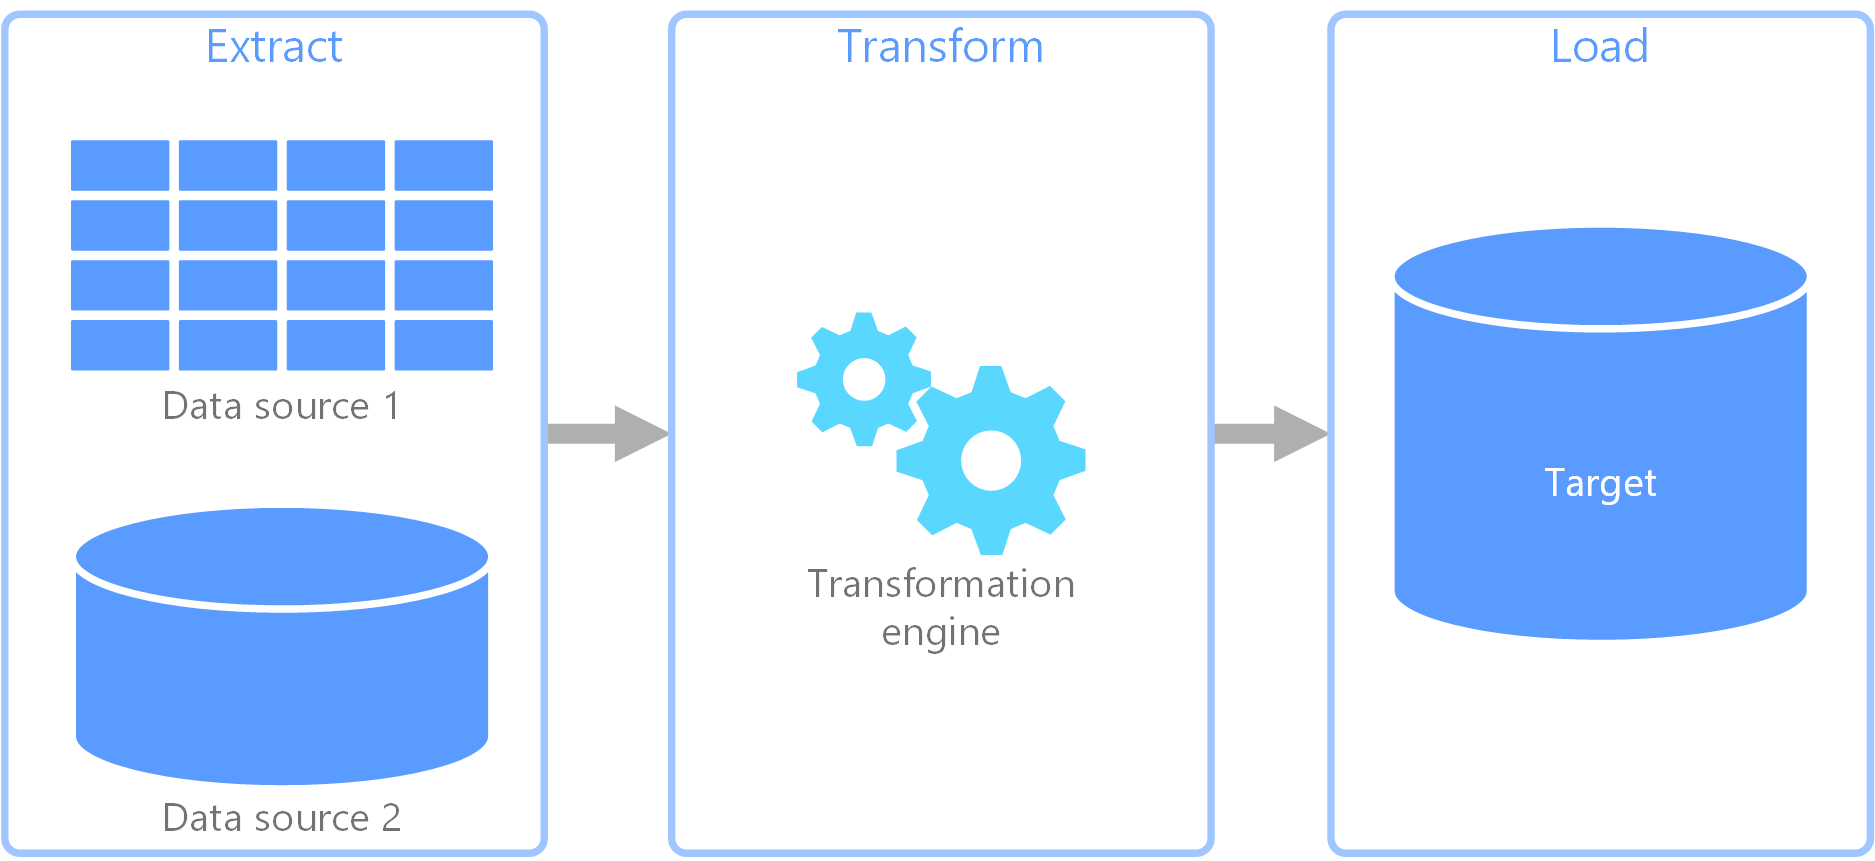
\includegraphics[width=0.80000\textwidth]{../images/etl.png}
\caption{Rappresentazione di un processo di ETL \label{figure_4}}
\end{figure}

Un processo di ETL si compone di tre parti:

La prima parte del processo di ETL è la fase di \textbf{Extract} ed
involve l'estrazione dei dati da più data sources come database
relazionali o non-relazionali, file JSON od XML ma anche risorse
``adhoc'' come, ad esempio, dei dati generati da programmi di web
analytics.

L'obiettivo di questa fase è estrarre tutti i dati necessari dalle
possibili sorgenti e prepararli alla fase di Transform.

Un importante problema legato a questa fase è il processo di
\emph{validazione delle sorgenti dati}: con più sorgenti dati spesso ci
si ritrova a dover gestire più formati non necessariamente compatibili
tra loro.\\
Per poter garantire alla fase di Transform dei dati comprensibili,
durante la fase di Extract vengono definite delle \emph{regole di
validazione} per filtrare i dati provenienti dalle varie sorgenti, un
esempio di regola di validazione è il controllo dei tipi di dati
presenti nella fonte.

\newpage

Nella fase di \textbf{Transform} una serie di regole e funzioni vengono
applicate ai dati generati dalla fase di Extract per prepararli alla
fase di Load nella data warehouse.

Il primo compito della fase di Transform è la \emph{pulizia dei dati}:
spesso le varie fonti di dati, nonostante siano state validate, possono
presentare incongruenze tra loro come caratteri speciali legati
all'encoding della propria sorgente oppure formati dei dati diversi ma
compatibili (un esempio può essere la differneza di formattazione tra
date americane ed europee).\\
Per garantire un corretto funzionamento delle operazioni di
trasformazione è quindi necessario pulire i dati ed adattarli ad un
formato comune.

Il secondo compito della fase di Transform è la \emph{trasformazione dei
dati} in nuovi dati richiesti dal business, esempi di trasformazioni
sono:

\begin{itemize}
\tightlist
\item
  Joining di tabelle da più sorgenti
\item
  Mapping e trasformazione di dati (esempio: ``Maschio'' in ``M'')
\item
  Aggregazione di dati
\item
  Generazione/calcolo di nuovi dati
\item
  Selezione di insiemi di dati
\item
  Validazione del nuovo formato di dati prodotto
\end{itemize}

Nella fase di \textbf{Load} l'insieme di dati generati dalla fase di
Transform vengono inseriti in un target, il quale potrebbe essere una
data warehouse ma anche più semplicemente un file in un formato utile.\\
Business diversi hanno necessità diverse, per questo l'implementazione
della fase di load può avere più modalità implementative, il punto
focale di questa fase è proprio stabilire la frequenza e le modalità di
aggiornamento dei dati presenti nel target.\\
Decidere la frequenza (giornaliera, mensile, ecc.) e le modalità
(sovrascrizione dei vecchi dati o meno) del target possono portare ad un
processo di ETL più o meno utile ad una azienda.

Per generare un buon target è buona norma definire uno schema
\emph{preciso e chiaro} della tipologia di dati a cui il target deve
aderire.\\
Come detto in precedenza un processo di ETL è utilizzato per aggregare
più fonti di informazioni comuni ad un processo aziendale, questo
suppone che le informazioni presenti nella data warehouse potrebbero
venire usate da più parti di una azienda, le quali potrebbero essere
abituate a particolari formati dei dati.\\
Senza definire uno schema dei dati chiaro e preciso, si correrebbe il
rischio di generare un insieme di dati inutilizzabile da determinati
reparti in quanto non conforme al formato di dati da loro conosciuto.

\newpage

\hypertarget{event-sourcing}{\subsection{4. Event
sourcing}\label{event-sourcing}}

\subsubsection{4.1. L'importanza dei dati e degli
eventi}\label{limportanza-dei-dati-e-degli-eventi}

Lo status quo delle moderne applicazioni web è basato sul utilizzo di
database per rappresentare le specifiche di dominio, spesso espresse da
un cliente e/o da un esperto del dominio esterno all'ambiente di
sviluppo.

Durante la fase di analisi dei requisiti (supponendo un modello di
sviluppo del software agile) cliente e team di sviluppo si confrontano,
cercando di trovare un linguaggio comune per definire la logica e
l'utilizzo del software richiesto; Una volta stabiliti i requisti, il
team di sviluppo generalmente inizia uno studio interno atto a produrre
un \emph{modello dei dati} che verrà usato come base per definire lo
schema dei database utilizzati dal sistema.\\
Un cliente comune molto spesso non ha padronanza del concetto di `stato
di una applicazione', ma piuttosto si limita ad esporre i propri
requisiti descrivendo i possibili eventi che, traslati sul modello di
sviluppo incentrato su i database, portano il team di sviluppo a
ragionare sui possibili stati di un database in risposta a questi
eventi.

Lo stato di un database di una applicazione è strettamente legato
all'insieme degli eventi del dominio applicativo; L'unico modo per
modificare o interagire con questo database è tramite i comandi di
inserimento, cancellazione o lettura, tutti comandi che vengono eseguiti
solamente all'avvenire di un particolare evento.

Un database mantiene solo lo stato corrente di una applicazione; Non
esiste il concetto di cronologia del database a meno di utilizzare
soluzioni basate su \textbf{Change Data Capture} (CDC), generalmente
utilizzate per generare un transactional log contenente tutte le
operazioni eseguite sul suddetto database.\\
In questo modello database-driven, un evento genera un cambiamento su
una base di dati; Gli eventi e lo stato di un database sono però
concetti diversi e slegati tra loro, l'esecuzione di un evento a volte
può portare ad una asincronia tra l'esecuzione di un evento e lo stato
di un database, tanto più se questo database è utilizzato da tutti i
microservizi di una applicazione.

Una soluzione al problema di più microservizi che utilizzano lo stesso
database è di utilizzare delle views del database locali ad ogni
microservizio: ogni servizio lavorerà su una copia locale del database
ed un job esterno si occuperà di compattare le views e mantenere il
database aggiornato rispetto a tutti i cambiamenti.\\
Questa soluzione ha un enorme problema: supponiamo di notare un errore
sul database e di doverlo correggere, come possiamo decidere quale delle
views è ``più corretta'' delle altre? Per aiutarci nella ricerca
dell'errore potremmo utilizzare il transactional log di ogni views, ma
su database di grandezze importanti esaminare il log di ogni views che
lo compone potrebbe essere un problema complesso e dispendioso in
termini di tempo.

Event sourcing propone di risolvere questo genere di problemi
allontanandosi da una progettazione state-driven elevando gli eventi a
elementi chiavi del modello dei dati di una applicazione.

\subsubsection{4.2. Descrizione}\label{descrizione}

Event sourcing (ES) è un design pattern che si contrappone ad una
visione del mondo basata sullo stato di una applicazione fornendo come
alternativa l'uso degli eventi, ovvero delle azioni o accadimenti che
l'applicazione è in grado di riconoscere e gestire.

Durante l'analisi dei requisiti di una applicazione, spesso ci si trova
a confronto con esperti di un dominio applicativo che non hanno
particolare conoscenza delle tecnologie necessarie per implementare le
loro richieste, è compito del programmatore (o del team di
programmatore) analizzare le sue richieste e trasformarle in idee
gestibili.\\
In genere questi esperti spiegheranno al programmatore le loro necessità
illustrando il funzionamento del dominio utilizzando concetti molto più
vicini a degli \emph{eventi} piuttosto che \emph{sequenze di
richieste/risposte a/da un database}; Supponendo di dover sviluppare una
piattaforma di e-commerce, è molto più probabile che l'esperto di
dominio richieda di gestire eventi come ``aggiungere un oggetto al
carrello'' oppure ``comprare un oggetto'' piuttosto che ``creare dei
database per gestire carrello, stock oggetti rimamenti, oggetti
comprati''.

La struttura dati fondamentale alla base di ES è l'\textbf{event store},
una tipologia di database ottimizzata per la gestione di eventi.\\
In un event store, gli eventi vengono inseriti in fondo alla struttura
in ordine di avvenimento e non possono essere modificati o cancellati;
Nel caso venga pubblicato per errore un evento sbagliato o inesatto per
annularlo basterà pubblicare un evento contrario. Questo meccanismo
garantisce che la ripetizione della storia degli eventi \emph{porterà
sempre allo stesso stato, errore compreso}.

Un event store è comunemente implementato utilizzando un \textbf{log},
una sequenza di record append-only e totalmente ordinata in base al
tempo di scrittura del record.

\begin{figure}
\centering
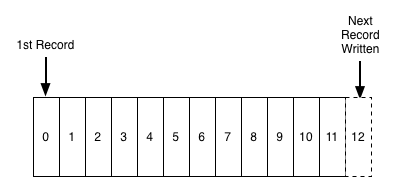
\includegraphics[width=0.68000\textwidth]{../images/log.png}
\caption{Struttura di un log \label{figure_1}}
\end{figure}

I record sono inseriti in fondo al log e il processo di lettura è
eseguito partendo dall'inizio del log.

Generalmente in un processo di sviluppo basato su ES, si tende a
nominare gli eventi con il tempo passato per esplicitare il concetto che
un evento è un avvenimento passato, un esempio nome per un evento
potrebbe essere \texttt{item\_created} oppure \texttt{item\_bought}.

L'ordine di pubblicazione degli eventi è di estrema importanza in quanto
è ciò che permette al pattern di rappresentare correttamente lo stato di
una applicazione.

E' possibile vedere lo stato corrente di una applicazione come una
\emph{sequenza di operazioni di modifica dello stato eseguite partendo
da uno stato iniziale}, questo implica che è possibile vedere un evento
come il \emph{delta tra lo stato iniziale di una applicazione e lo stato
corrente dell'applicazione dopo l'esecuzione dell'evento}.\\
La possibilità di trasformare lo stato corrente di una applicazione in
una funzione dello stato iniziale dell'applicazione e una sequenza di
eventi è il meccanismo che permette ad event sourcing di avere una
validità tecnica per la gestione dei dati di una applicazione.

\begin{figure}
\centering
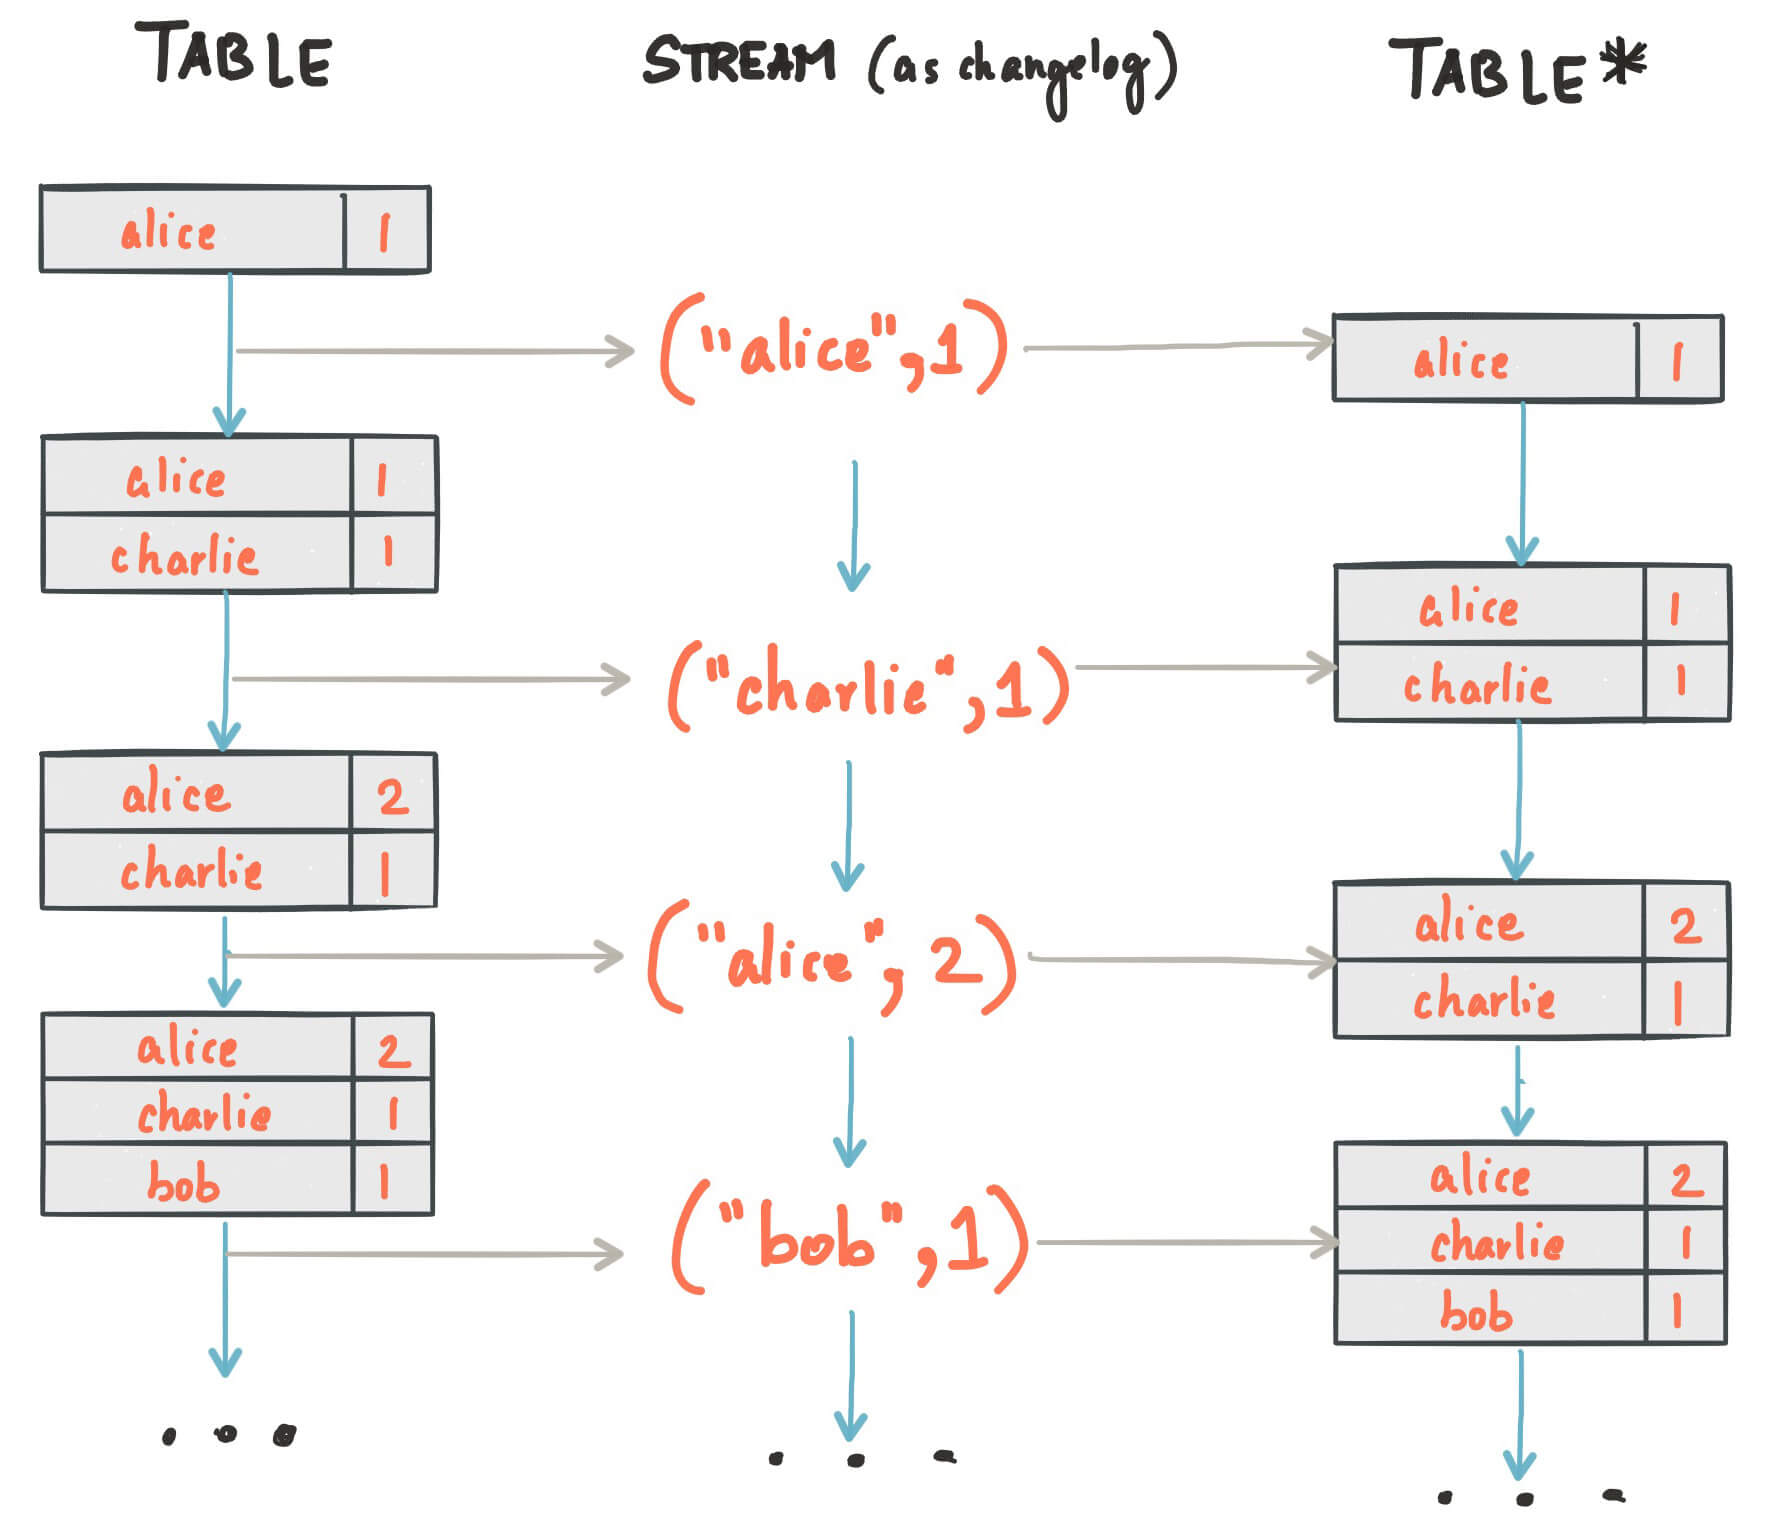
\includegraphics[width=0.80000\textwidth]{../images/streams-table-duality.jpg}
\caption{Dualità tra stream e database \label{figure_2}}
\end{figure}

\newpage

\subsubsection{4.3. Vantaggi}\label{vantaggi}

Event sourcing è un pattern estremamente utile per tutti quegli use-case
dove è assolutamente necessario mantenere una storia dello sviluppo
dello stato dell'applicazione del tempo. Tipici esempi sono gli
strumenti di versioning del codice oppure la gestione di un storico
bancario.

La capacità dell'event store di essere sia una struttura dati
performante per la scrittura dei dati (è una semplice operazione di
scrittura in fondo ad una sequenza di complessità O(1)) che una
cronologia di tutti gli avvenimenti del sistema, permette una gestione
degli errori estremamente semplice.

In un qualsiasi database relazionale se durante il normale utilizzo
dell'applicazione avviene un errore logico che porta il database ad uno
stato non corretto, è sempre necessario un rollback dell'intero database
ad un data antecedente l'errore per poter sperare di correggiare
l'errore.\\
Tale processo è dispendioso in termini di tempo e non è di facile
esecuzione in quanto spesso il processo di backup di un database non
viene eseguito dopo ogni inserimento o update di un record; Per poter
correggere l'errore sarà quindi necessario calcolare partire dal backup
più recente e applicare nuovamente tutte le transformazioni del
database, meno l'errore.

L'analisi del motivo dell'errore può inoltre non essere di facile
realizzazione con un database relazionale a meno che non siano in uso i
meccanismi di CDC: senza una cronologia delle transazioni può essere
molto difficile risalire al motivo dell'errore.

Diversamente nel caso dell'utilizzo di Event Sourcing, la gestione e
l'analisi di un errore è estremamente semplice. Nel caso in cui
l'errore, che sarà sempre un evento, non ha generato un effetto
``domino'' sul sistema (ovvero l'errore non ha portato all'esecuzione di
uan catena di errori), una volta individuato è possibile pubblicare un
evento ``contrario'' alla causa dell'errore in modo tale da cancellare
l'apporto dell'errore sul sistema.\\
Nel caso contrario, ovvero il caso in cui l'errore ha generato una
sequenza di errori, per ottenere lo stato corretto del sistema basterà
ripetere l'esecuzione di tutti gli eventi del sistema escludendo quello
che ha generato l'errore sulla base di dati.

E' bene notare che con ES la gestione degli errori nello stato del
sistema è strettamente legata all'atomicità e definizione degli eventi
del sistema: una corretta (semplice) definizione degli eventi del
sistema porterà ad una cronologia del sistema più chiara e
comprensibile.

\newpage

\subsubsection{4.4. Svantaggi}\label{svantaggi}

Event sourcing potrebbe non essere utile per una applicazione che
richiede frequenti e continue query di richiesta sullo stato del
sistema.

Come descritto in precedenza, per ottenere lo stato corrente del sistema
è necessario eseguire tutti gli eventi pubblicati sull'event store
partendo da uno stato iniziale; Se la nostra applicazione richiede di
eseguire molte query di ricerca sullo stato corrente del database sarà
quindi necessario calcolare lo stato del sistema \emph{ogni volta che
viene eseguita una nuova richiesta} (un esempio di richiesta sullo stato
è la ricerca di tutti i record che presentano una particolare
caratteristica).

Le modalità per risolvere questo problema sono determinate dal dominio e
uso dell'applicazione che utilizza ES, ma generalmente per ovviare a
questa debolezza vengono realizzati degli snapshot dello stato
dell'applicazione da utilizzare per l'esecuzione delle query di
ricerca.\\
La frequenza di generazione ed aggiornamento di questi snapshot è
strettamente legata al dominio applicativo dell'applicazione.

\newpage

\subsection{5. Apache Kafka: Ecosistema}\label{apache-kafka-ecosistema}

\subsubsection{5.1. Introduzione}\label{introduzione-1}

\emph{Publish/Subscribe} è un pattern architetturale utilizzato per la
comunicazione asincrona tra diversi processi od oggetti.

In questo schema mittenti e destinatari dialogano tra loro per mezzo di
un \emph{broker}, un processo incaricato, da una parte, di ricevere
messaggi da dei mittenti e dall'altra di consegnare gli stessi messaggi
a dei destinatari.

I destinatari non conoscono i mittenti, ed i mittenti non si interessano
di chi sono i destinatari: l'unico compito del mittente è quello di
pubblicare dei messaggi sul broker, starà poi al destinatario il compito
di abbonarsi (dall'inglese \emph{subscribe}) al broker in modo da
ricevere tutti i nuovi messaggi.

Questo pattern viene spesso utilizzato quando ci si trova ad avere più
processi o servizi che generano delle metriche o dei dati, i quali sono
di vitale importanza per altrettanti servizi.

Una soluzione alternativa sarebbe creare dei canali dedicati tra
produttori e consumatori ma questo non permetterebbe alla struttura di
supportare un numero sempre più elevato di servizi od oggetti, ed in un
mondo dove è sempre più frequente l'utilizzo di microservizi e il
logging di eventi e dati (Big Data) porterebbe ad un debito tecnologico
elevato e difficile da correggere.

E' in questo contesto che nasce Apache Kafka, una \emph{streaming
platform} basata su un append-only log utilizzato da dei \emph{producer}
per pubblicare dei messaggi consumati da dei \emph{consumer}.\\
I messaggi pubblicati vengono persistiti nel tempo, sono leggibili
deterministicamente da qualsiasi consumer ed distributi all'interno del
sistema secondo particolari logiche in modo da garantire protezione da
crash e scalabità del sistema.

\newpage

\subsubsection{5.2. Messaggi}\label{messaggi}

L'unità dati fondamentali in Kafka è chiamata \emph{messaggio} o
\emph{record}.

Ogni messaggio è suddiviso in \emph{key} (opzionale) e \emph{value} e
possono essere di qualsiasi formato; Kafka non impone particolari
standard riguardo i formati dei dati utilizzabili all'interno del
sistema ma con lo scorrere del tempo \emph{Avro} è diventato lo standard
de facto.

Il campo \texttt{key}, quando definito, è un byte array utilizzato come
metadata per garantire un particolare ordinamento all'interno di un
\emph{topic}, un altro elemento fondamentale dell'architettura.

Nonostante Kafka sia una streaming platform, la scrittura e propagazione
dei messaggi all'interno della rete non avviene necessariamente per
messaggio, invece, piccoli gruppi di messaggi diretti verso la stesso
topic vengono raggruppati in \emph{batches}.

La gestione dei messaggi in batch nasce per motivi di efficienza per
bilanciare throughput e latenza: a fronte di una latenza più alta per la
consegna di un batch, vengono sprecate meno le risorse del sistema che
altrimenti si ritroverebbe costretto a gestire l'overhead di conoscegna
di un batch per ogni singolo messaggio.

\newpage

\subsubsection{5.3. Topic e partizioni}\label{topic-e-partizioni}

Un \emph{topic} è un elemento utilizzato in Kafka per categorizzare una
collezione di messaggi, e consiste in un unico stream di dati.

Un topic è suddiviso in \emph{partizioni}, append-only logs sui quali
vengono persisti i messaggi generati dai \emph{producers}.

\begin{figure}
\centering
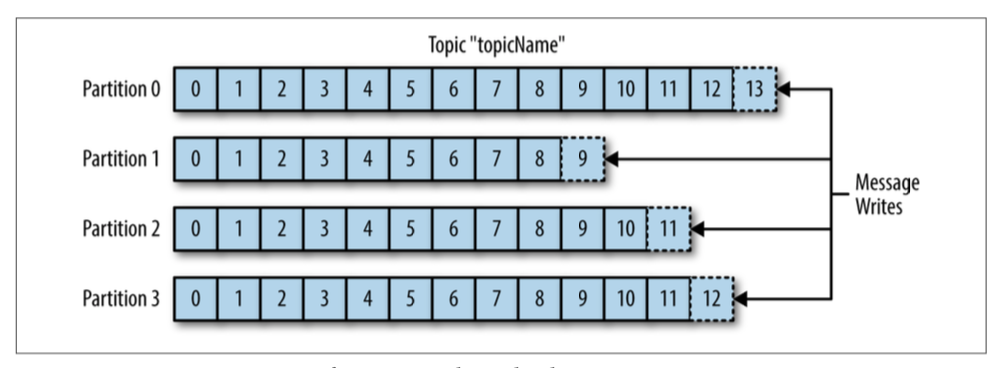
\includegraphics[width=0.90000\textwidth]{../images/topic-and-partitions.png}
\caption{Un topic suddiviso in più partizioni \label{figure_3}}
\end{figure}

I messaggi sono inseriti in una partizione da un producer nell'ordine in
cui sono stati inviati posizionandoli in fondo al log, non sono
modificabili o cancellabili e sono contradistinti da un \emph{offset},
un indice numerico che funziona da timestamp del messaggio. Un consumer
legge i messaggi di un topic partendo dalla testa (o da uno specifico
offset) del log proseguendo fino alla coda.

L'ordine di scrittura è garantito solo per ogni singola partizione: non
è detto che messaggi appartenenti al medesimo topic siano in ordine
cronologico se inseriti su partizioni diverse.

Per dare un esempio pratico di topic, supponiamo di utilizzare Kafka per
creare uno storage di eventi ricevuti dal front-end di una applicazione:
tipici eventi che vengono spesso loggati da un front-end possono essere
\emph{i link cliccati in una pagina}, \emph{quali pagine sono state
visualizzate in una sessione} oppure \emph{se è stato visualizzato un
particolare video embdeed}.

Per ogniuno di questi eventi verrà creato un singolo \texttt{topic} per
raggruppare tutte le notifiche e dati generati da uno di quei
particolari eventi a front-end: ad esempio avremo il topic
\texttt{views-video-embdeed} sul quale verranno registrati dei semplici
\texttt{yes} o \texttt{no} con magari l'aggiunta di un
\texttt{timestamp} (l'ora di visualizzazione), in questo modo il topic
ci permetterà di calcolare la frequenza di visualizzazione del video.

\newpage

\subsubsection{5.4. Producers}\label{producers}

Kafka è utilizzata da due tipologie di client: \emph{producers} e
\emph{consumers}.

I \emph{producers} hanno il compito di creare messaggi indirizzati a
specifici topic (indipendentemente dal numero di partizioni da cui sono
formati).\\
Come illustrato in precedenza, un topic è formato da un numero variabile
di partizioni utilizzate come meccanismo di replica e gestione dei
messaggi; Alla creazione di un messaggio è possibile indicare al
producer su quale partizione andare a scrivere il record specificando
l'identificativo di una partizione specifica.

\begin{figure}
\centering
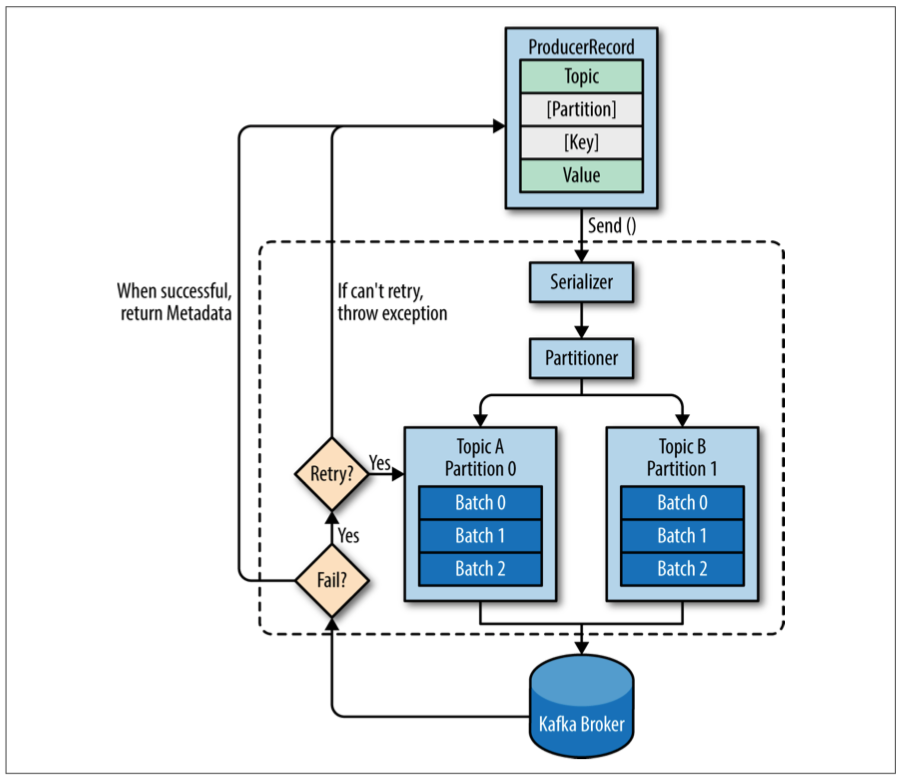
\includegraphics[width=0.90000\textwidth]{../images/producer-process.png}
\caption{Processo di pubblicazione di un messaggio \label{figure_3}}
\end{figure}

Il processo di pubblicazione di un messaggio inizia con la produzione di
un \texttt{ProducerRecord} il quale deve contenere il topic sul quale
vuole pubblicare il messaggio ad una value, ovvero il contenuto del
messaggio; Opzionalmente è possibile specificare una chiave o una
partizione specifica.

Nella maggior parte dei casi d'uso di Kafka, il producer non si pone mai
il problema di decidere su quale partizione andare a scrivere un
particolare messaggio ma piuttosto vengono utilizzati dei meccanismi di
load-balancing per spartire correttamente i messaggi su tutte le
partizioni disponibili presenti nel topic.\\
Tipici esempi di algoritmi di load-balancing sono il calcolo della
partizione in base ad una hash key derivata dall'offset del messaggio
oppure utilizzando un algoritmo round robin, se necessario è presente la
possibilità di specificare un \emph{partioneer} creato su misura al caso
d'uso.

Una volta creato il \texttt{ProducerRecord} il producer serializza
chiave e value del messaggio in \texttt{ByteArray} in modo da
effettivamente trasmetterli sulla rete. I dati sono quindi recapitati ad
un partitioner che andrà a deciderà su quale partizione pubblicare il
messaggio (solo nel caso in cui la partizione non era già stata
specificata nel record). Il record viene quindi aggiunto ad un batch di
record e il producer resta in attesa di avere abbastanza record (o
alternativamente, in attesa della scadenza di un timeout) prima di
inviare il batch di messaggi ad un broker.

Una volta che il broker riceve il batch di messaggi verranno effettuati
una serie di controlli per garantire la validità dei messaggi del batch
rispetto al topic su cui si sta cercando di pubblicare questi messaggi;
In caso positivo il broker invia al producer un \texttt{RecordMedatada}
con topic, partizione e offset dei messaggi dei pubblicati, altrimenti
ritornerà un errore. In caso di errore, il producer può provare a
rinviare il batch di messaggi.

Ogni partizione in un cluster ha un \emph{leader} ed un insieme di sue
\emph{repliche} distribuite sui vari brokers.

Tutte le pubblicazioni dirette ad una particolare partizione devono
prima essere pubblicate sul leader, ed in un secondo momento devo
essereno replicate sulle repliche (o followers), questo meccanismo è
utilizzato per garantire la durabilità dei dati in un cluster: se uno
dei leader muore, viene eletta una delle repliche a nuovo leader della
partizione e viene creata una nuova replica.

E' possibile garantire diversi livelli di durabilità a seconda di come
viene configurato il producer, favorendo od evitando problemi di
scrittura e lettura dei messaggi a scapito del throughput.

\newpage

Per poter creare un producer sono necessari tre parametri:

\begin{itemize}
\tightlist
\item
  \texttt{bootstrap.servers}: lista degli indirizzi (\texttt{host:port})
  dei brokers del cluster Kafka che vogliamo utilizzare.
\item
  \texttt{key.serializer}: nome della classe che verrà utilizzata per
  serializzare in byte array le chiavi dei record che vogliamo
  pubblicare con kafka. E' possibile crearne di nuovi implementando
  \texttt{org.apache.kafka.common.serialization.Serializer}.
\item
  \texttt{value.serializer}: nome della classe che verrà utilizzata per
  serializzare in byte array il record da pubblicare.
\end{itemize}

Un esempio di producer è dato dal seguente codice Scala:

\small  

\begin{Shaded}
\begin{Highlighting}[]
\KeywordTok{import}\NormalTok{ java.}\FunctionTok{util}\NormalTok{.}\FunctionTok{Properties}
\KeywordTok{import}\NormalTok{ org.}\FunctionTok{apache}\NormalTok{.}\FunctionTok{kafka}\NormalTok{.}\FunctionTok{clients}\NormalTok{.}\FunctionTok{producer}\NormalTok{.\{Callback, RecordMetadata\}}
\KeywordTok{import}\NormalTok{ org.}\FunctionTok{apache}\NormalTok{.}\FunctionTok{kafka}\NormalTok{.}\FunctionTok{clients}\NormalTok{.}\FunctionTok{producer}\NormalTok{.\{ProducerRecord, KafkaProducer\}}
\KeywordTok{import}\NormalTok{ scala.}\FunctionTok{concurrent}\NormalTok{.}\FunctionTok{Promise}

\KeywordTok{case} \KeywordTok{class} \FunctionTok{Producer}\NormalTok{(topic: String)\{}
    \KeywordTok{val}\NormalTok{ props = }\KeywordTok{new}\NormalTok{ Properties()}
\NormalTok{    props.}\FunctionTok{put}\NormalTok{(}\StringTok{"bootstrap.servers"}\NormalTok{, }\StringTok{"localhost:9092"}\NormalTok{)}
\NormalTok{    props.}\FunctionTok{put}\NormalTok{(}\StringTok{"key.serializer"}\NormalTok{, }
        \StringTok{"org.apache.kafka.common.serialization.StringSerializer"}\NormalTok{)}
\NormalTok{    props.}\FunctionTok{put}\NormalTok{(}\StringTok{"value.serializer"}\NormalTok{, }
        \StringTok{"org.apache.kafka.common.serialization.StringSerializer"}\NormalTok{)}
    
    \KeywordTok{private} \KeywordTok{val}\NormalTok{ producer = }\KeywordTok{new}\NormalTok{ KafkaProducer[String, String](props)    }
    
    \KeywordTok{def} \FunctionTok{send}\NormalTok{(value: String) = \{}
      \KeywordTok{val}\NormalTok{ record = }\KeywordTok{new}\NormalTok{ ProducerRecord[String, String](topic, value)}

      \KeywordTok{try}\NormalTok{ \{}
\NormalTok{        producer.}\FunctionTok{send}\NormalTok{(record).}\FunctionTok{get}\NormalTok{()}
\NormalTok{      \} }\KeywordTok{catch}\NormalTok{ \{}
        \KeywordTok{case}\NormalTok{ e: Exception => e.}\FunctionTok{printStackTrace}
\NormalTok{      \}}
\NormalTok{    \}   }

    \KeywordTok{def} \FunctionTok{sendAsync}\NormalTok{(value: String) = \{}
        \KeywordTok{val}\NormalTok{ record = }\KeywordTok{new}\NormalTok{ ProducerRecord[String, String](topic, value)}
        \KeywordTok{val}\NormalTok{ promise = Promise[(RecordMetadata, Exception)]()}

\NormalTok{        producer.}\FunctionTok{send}\NormalTok{(record, }\KeywordTok{new}\NormalTok{ Callback \{}
            \KeywordTok{override} \KeywordTok{def} \FunctionTok{onCompletion}\NormalTok{(metadata: RecordMetadata, }
\NormalTok{                                      exception: Exception) = \{}
\NormalTok{                promise.}\FunctionTok{success}\NormalTok{((metadata, exception))}
\NormalTok{            \}}
\NormalTok{        \})}
\NormalTok{    \}}
\NormalTok{\}}
\end{Highlighting}
\end{Shaded}

\normalsize
\newpage

Creato un oggetto \texttt{Properties} con le configurazioni di base,
viene creato un nuovo producer capace di pubblicare dei record (di tipo
\texttt{String}) ad un topic (passato come parametro alla case class)
con il metodo \texttt{send(value:\ String)}.

Un producer può inviare record con tre diverse modalità:

\begin{itemize}
\tightlist
\item
  \textbf{Fire-and-forget}: il messaggio viene mandato al server e viene
  ignorata la possibilità che questo messaggio non venga ricevuto.
\item
  \textbf{Sincrona}: il messaggio viene mandato con un metodo
  \texttt{send()} il quale restituisce un \texttt{Future}, viene quindi
  utilizzato il metodo \texttt{.get()} per attendere una risposta dal
  server per capire se il messaggio è effettivamente stato ricevuto.
\item
  \textbf{Asincrona}: il metodo \texttt{send()} restituisce una
  \texttt{callback} che verrà eseguita quando (e se) riceverà una
  risposta dal broker Kafka.
\end{itemize}

E' possibile configurare un producer
\href{https://kafka.apache.org/documentation.html\#producerconfigs}{secondo
una moltitudine di campi di configurazione}, ma sicuramente uno dei più
importanti è il valore attribuito al campo \texttt{acks} il quale è
direttamente collegato alla durabilità dei messaggi e definisce quante
repliche devono ricevere il messaggio pubblicato sul leader prima di
poter garantire al producer la corretta pubblicazione del messaggio.

Esistono tre possibili valori per \texttt{acks}:

\begin{itemize}
\tightlist
\item
  con \texttt{acks=0}, il producer non si aspetterà di ricevere un
  messaggio di conferma da parte del broker. Questo implica che nel caso
  di un malfunzionamento, il producer non sarà a conoscenza del
  fallimento ed il messaggio verrà perso. E' l'opzione che garantisce il
  più alto valore di throughput.
\item
  con \texttt{acks=1}, il producer riceverà un messaggio di conferma di
  pubblicazione del messaggio appena \emph{almeno} una replica
  confermerà di aver ricevuto il messaggio pubblicato sul leader. Con
  questa opzione è comunque possibile perdere il messaggio se, a seguito
  della morte del leader, viene eletto come nuovo leader non la replica
  che aveva confermato la ricezione del messaggio ma piuttosto una delle
  repliche che non lo avevano ancora ricevuto.
\item
  con \texttt{acks=all}, il producer riceverà conferma della
  pubblicazione del messaggio solo dopo che tutte le repliche hanno
  ricevuto il messaggio pubblicato sul leader. Questa opzione garantisce
  la pubblicazione di un messaggio a scapito di un minor throughput.
\end{itemize}

\newpage

\subsubsection{5.5. Consumers}\label{consumers}

Un \emph{consumer} è un client Kafka utilizzato per leggere dati da un
topic e tipicamente è parte di un \emph{consumer group}.\\
Un consumer group è definito da uno specifico \texttt{group.id} ed un
topic che tutti i membri del gruppo hanno in comune; Ogni partizione del
topic è letta da un solo consumer del gruppo e più consumer del gruppo
non possono leggere dalla stessa partizione.\\
Supponiamo di avere un topic T1 con quattro partizioni, nel caso in cui
il nostro gruppo è formato da un solo consumer C1 sarà solo lui a
consumare l'intero topic.

\begin{figure}
\centering
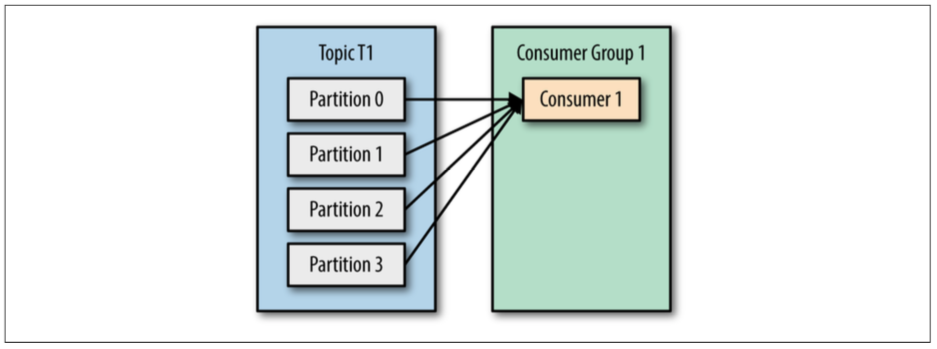
\includegraphics[width=1.00000\textwidth]{../images/single-consumer.png}
\caption{Un consumer con quattro partizioni \label{figure_3}}
\end{figure}

Se aggiungiamo un nuovo consumer C2 al gruppo, ogni consumer riceverà
dati da solo due partizioni disponibili.

\begin{figure}
\centering
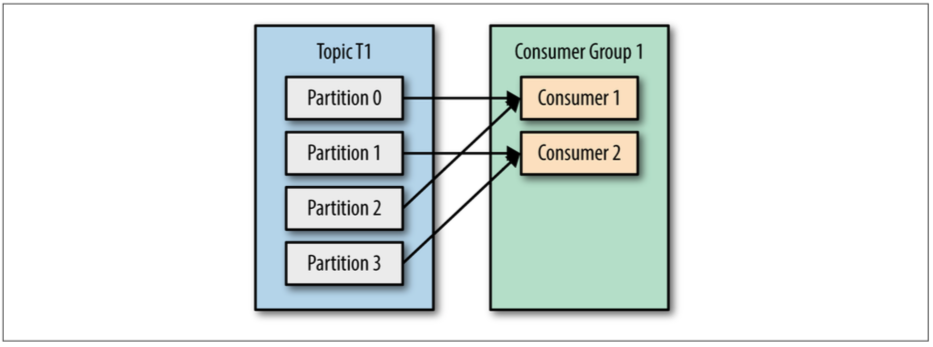
\includegraphics[width=1.00000\textwidth]{../images/two-consumers.png}
\caption{Due consumer consumano le quattro partizioni \label{figure_3}}
\end{figure}

\newpage

Con quattro consumer, ogni consumer leggerà da una sola partizione.

\begin{figure}
\centering
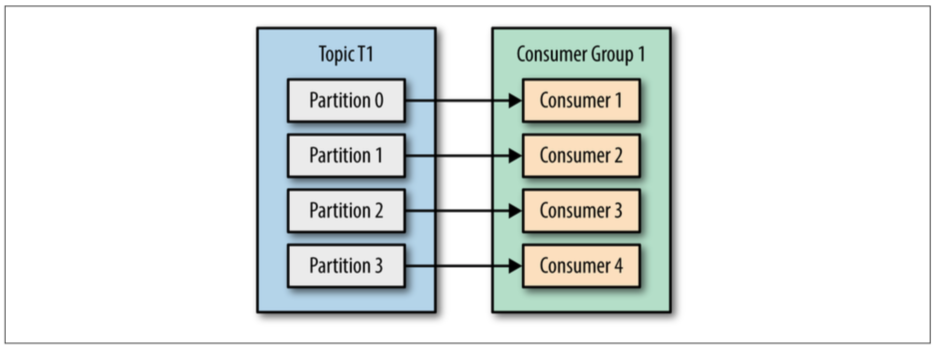
\includegraphics[width=1.00000\textwidth]{../images/four-consumers.png}
\caption{Quattro consumer consumano l'intero topic individualmente
\label{figure_3}}
\end{figure}

Ed infine, nel caso in cui il gruppo contenga più consumer del numero di
partizioni del topic vi saranno sicuramente dei consumer che non
leggeranno dal topic.

\begin{figure}
\centering
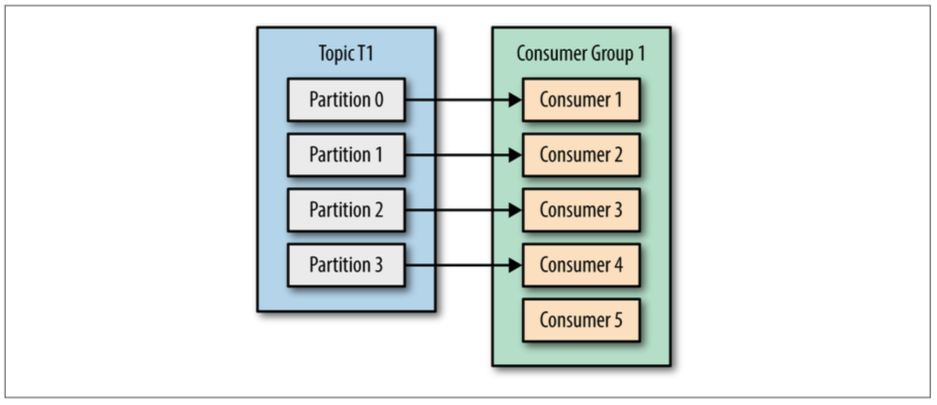
\includegraphics[width=1.00000\textwidth]{../images/five-consumers.png}
\caption{Un numero troppo elevato di consumer rispetto alle partizioni
di un topic \label{figure_3}}
\end{figure}

Questo meccanismo di bilanciamento dei consumer rispetto alle partizioni
di un topic permette di scalare l'architettura orizzontalmente nel caso
di topic con grossi moli di dati sensibili che necessitano di essere
consumati da applicazioni con operazioni ad alta latenza come la
scrittura su un database o l'esecuzione di calcoli: con Kafka, per
evitare situazioni a ``collo di bottiglia'', basta aumentare il numero
di partizioni di un topic ed il numero di consumer di quel particolare
topic.

Un altro importante vantaggio dell'utilizzo dei consumer group è dato
dalla possibilità di ribilanciare il gruppo nel caso di crash, morte o
aggiunta di un consumer.\\
Per \emph{ribilanciare il consumer group} si intende il processo di
cambio di proprietà di una partizione da un consumer A ad un consumer B;
Questo procedimento, insieme alla possibilità di aggiungere e rimuovere
consumer per ogni partizione, è ciò permette a Kafka di scalare la
propria architettura su grossi numeri di record e topic. E' importante
notare che questa funzionalità non è comunque desiderabile: durante un
rebalance il consumer group non può consumare i dati di un topic,
comportando quindi un rallentamento nella lettura dei dati.

Un consumer per non risultare morto deve inviare degli \emph{heartbeats}
al broker eletto a \emph{cordinator} del consumer group. Questi ``segni
di vita'' sono inviati al broker ogni volta che il consumer tenta di
leggere dal topic.

Nel caso in cui il broker non riceva un heartbeat da un consumer entro
un particolare lasso di tempo, verrà subito scatenato un ribilanciamento
del gruppo a cui appartiene il consumer. Allo stesso modo, nel caso in
cui un consumer venga rimosso dal gruppo, sarà lo stesso consumer ad
inviare un messaggio di ``uscita'' dal gruppo al broker che anche in
questo caso forzerà un ribilanciamento del consumer group.

Un esempio di consumer sviluppato in Scala è dato dal seguente codice:

\begin{Shaded}
\begin{Highlighting}[]

\KeywordTok{import}\NormalTok{ java.}\FunctionTok{util}\NormalTok{.}\FunctionTok{Properties}
\KeywordTok{import}\NormalTok{ org.}\FunctionTok{apache}\NormalTok{.}\FunctionTok{kafka}\NormalTok{.}\FunctionTok{clients}\NormalTok{.}\FunctionTok{consumer}\NormalTok{.}\FunctionTok{KafkaConsumer}

\KeywordTok{case} \KeywordTok{class} \FunctionTok{Consumer}\NormalTok{(topic: String)\{}
    \KeywordTok{val}\NormalTok{ props = }\KeywordTok{new}\NormalTok{ Properties()}
\NormalTok{    props.}\FunctionTok{put}\NormalTok{(}\StringTok{"bootstrap.servers"}\NormalTok{, }\StringTok{"localhost:9092"}\NormalTok{)}
\NormalTok{    props.}\FunctionTok{put}\NormalTok{(}\StringTok{"key.deserializer"}\NormalTok{, }
        \StringTok{"org.apache.kafka.common.serialization.StringSerializer"}\NormalTok{)}
\NormalTok{    props.}\FunctionTok{put}\NormalTok{(}\StringTok{"value.deserializer"}\NormalTok{, }
        \StringTok{"org.apache.kafka.common.serialization.StringSerializer"}\NormalTok{)}
\NormalTok{    props.}\FunctionTok{put}\NormalTok{(}\StringTok{"group.id"}\NormalTok{, }\StringTok{"example"}\NormalTok{)    }
    
    \KeywordTok{private} \KeywordTok{val}\NormalTok{ consumer = }\KeywordTok{new}\NormalTok{ KafkaConsumer[String, String](props)    }
\NormalTok{    consumer.}\FunctionTok{subscribe}\NormalTok{(util.}\FunctionTok{Collections}\NormalTok{.}\FunctionTok{singletonList}\NormalTok{(topic))}

    \KeywordTok{def} \FunctionTok{readTopic}\NormalTok{()\{}
        \KeywordTok{while}\NormalTok{(}\KeywordTok{true}\NormalTok{)\{}
            \KeywordTok{val}\NormalTok{ records = consumer.}\FunctionTok{poll}\NormalTok{(}\DecValTok{100}\NormalTok{)}
            \KeywordTok{for}\NormalTok{ (r <- records.}\FunctionTok{asScala}\NormalTok{)\{}
                \FunctionTok{println}\NormalTok{(s}\StringTok{"$\{r.offset\} $\{r.key\} $\{r.value\}"}\NormalTok{) }
\NormalTok{            \}}
\NormalTok{        \}}
\NormalTok{    \}}
\NormalTok{\}}
\end{Highlighting}
\end{Shaded}

\newpage

Come in precedenza con l'implementazione del producer, prima di poter
creare un producer è necessario definire alcune configurazioni minime:

\begin{itemize}
\tightlist
\item
  \texttt{bootstrap.servers}: l'indirizzo del broker
\item
  \texttt{key.deserializer}: il tipo di classe da utilizzare per
  deserializzare la chiave dei dati pubblicati su un topic
\item
  \texttt{value.deserializer}: il tipo di classe da utilizzare per
  deserializzare i dati pubblicati su un topic
\item
  \texttt{group.id}: l'identificativo del consumer group di cui il
  consumer fa parte
\end{itemize}

I consumer leggono i dati di un topic attraverso un meccanismo di
``pull'', ovvero sono loro stessi a richiedere al broker i dati.\\
Ogni volta che un consumer decide di leggere da un topic è lui stesso a
tenere traccia dell'ultimo messaggio che è stato letto e per tenerne
traccia utilizzerà un \emph{offset}: un identificativo corrispondente
alla posizione del messaggio nella partizione (il primo messaggio avrà
offset pari a 0, l'n-esimo messaggio offset n, etc.).

Dato che sono gli stessi consumer a tenere traccia dell'offset dei
messaggi letti e che sono sempre loro a richiedere i dati al broker
consumer group diversi possono leggere lo stesso topic senza perdita di
messaggi dal topic: i record presenti in un topic sono immutabili.

\begin{figure}
\centering
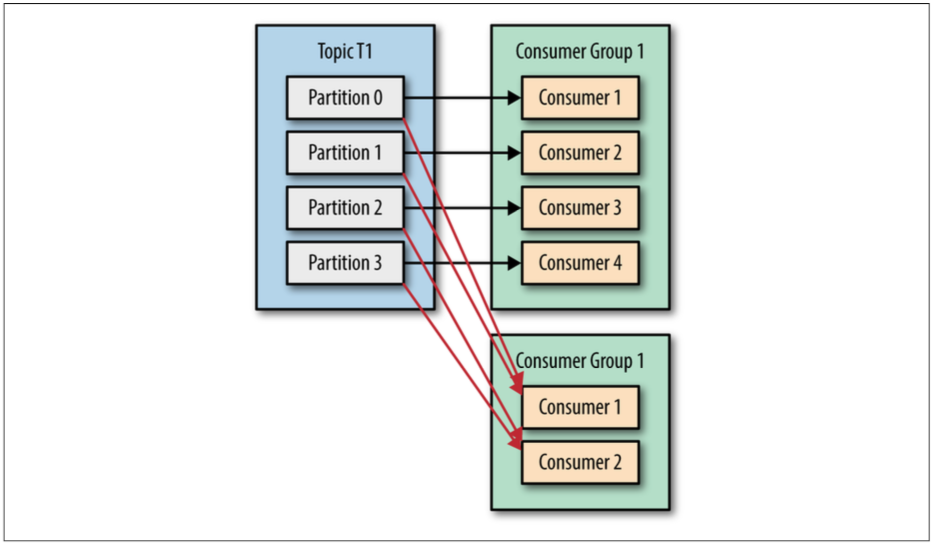
\includegraphics[width=1.00000\textwidth]{../images/consumer-groups.png}
\caption{Un topic con più gruppi di consumer \label{figure_3}}
\end{figure}

La lettura di una partizione può partire o dal primo messaggio esistente
oppure specificando un particolare offset.

Come si può vedere dalla funziona \texttt{readTopic()} definita
nell'esempio, un consumer utilizza un loop infinito di chiamate a
\texttt{.poll()} definito su un intervallo di tempo variabile (ovvero il
metodo messo a disposizione dall'interfaccia di Kafka) per richiedere al
broker tutti i messaggi che quel consumer non ha ancora letto.\\
Per sapere quali messaggi inviare il broker deve riceve dal consumer
l'offset dell'ultimo messaggio letto attraverso una operazione di
\_commit; Gli offset vengono pubblicati dai consumer su di uno speciale
topic Kafka chiamato \texttt{\_\_consumer\_offset} al quale tutti i
broker hanno accesso e a cui fanno riferimento per calcolare quali
messaggi inviare.

Il topic \texttt{\_\_consumer\_offset} è inoltre utilizzato nel caso di
ribilanciamento di un gruppo.\\
A seguito di un ribilanciamento un o più consumer del gruppo possono
ricevere un nuovo insieme di partizioni, e per capire da dove iniziare
il nuovo processo di lettura, devono interrogare il topic
\texttt{\_\_consumer\_offset}.

Se l'offset pubblicato su \texttt{\_\_consumer\_offset} è \emph{minore}
dell'offset dell'ultimo messaggio che il consumer client ha in memoria,
tutti i messaggi compresi tra i due offset verranno riprocessati.

\begin{figure}
\centering
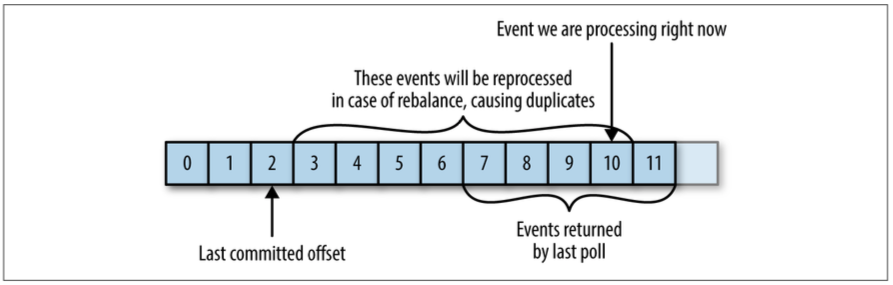
\includegraphics[width=1.00000\textwidth]{../images/early-offset.png}
\caption{Replay dei messaggi in base all'offset \label{figure_3}}
\end{figure}

Se l'offset pubblicato su \texttt{\_\_consumer\_offset} è
\emph{maggiore} dell'offset dell'ultimo messaggio che il consumer client
ha in memoria, tutti i messaggi compresi tra i due offset verranno
\emph{persi}.

\begin{figure}
\centering
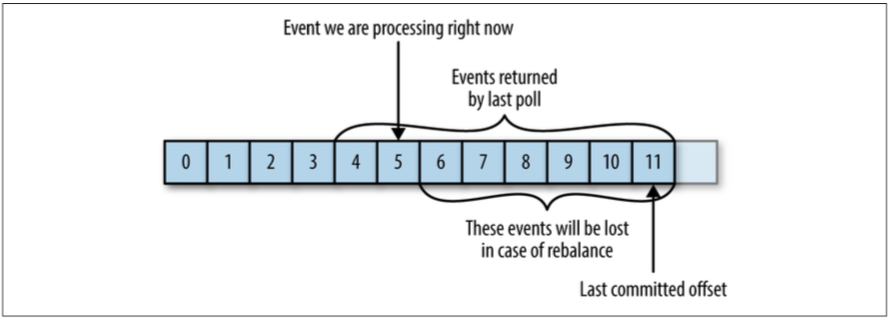
\includegraphics[width=1.00000\textwidth]{../images/late-offset.png}
\caption{Perdita di messaggi in base all'offset \label{figure_3}}
\end{figure}

Per una corretta gestione dei messaggi è quindi di assoluta importanza
la capacità di gestire gli offset in modo adeguato alle necessità di
ogni progetto, per questo motivo esistono varie possibile configurazione
del processo di commit:

\begin{itemize}
\tightlist
\item
  automatic commit: ogni cinque secondi il consumer genera un commit
  dell'ultimo offset letto con \texttt{.poll()}, è la configurazione di
  default di ogni consumer.
\item
  commit current offset: è lo stesso consumer a decidere quando inviare
  l'ultimo offset letto attraverso l'uso della funzione
  \texttt{commitSync()}: alla chiamata della funzione viene inviato al
  broker l'ultimo offset letto da \texttt{.poll()} ed il consumer rimane
  in attesa di un segnale di \texttt{acknowledgment} da parte del
  broker, in caso positivo il consumer continuerà nel processo di
  lettura, altrimenti verrà lanciata un'eccezione. E' prevista la
  possibilità di riprovare un numero di volte il processo di commit.
\item
  commit current offset in modalità asincrona: come la modalità
  precedente ma non bloccante per il consumer, l'offset viene inviato
  chiamando .commitAsync().
\end{itemize}

\subsubsection{5.6. Brokers e clusters}\label{brokers-e-clusters}

Un \emph{broker} è un server Kafka con svariati compiti quali ricevere,
indicizzare e salvare i messaggi inviati dai producers ed inviare i
messaggi richiesti dai consumers; Un singolo broker è capace di gestire
migliaia di partizioni e millioni di messaggi al secondo.

I broker sono stati creati per lavorare in \emph{clusters} ovvero gruppi
di brokers ordinanti secondo una particolare gerarchia.

\begin{figure}
\centering
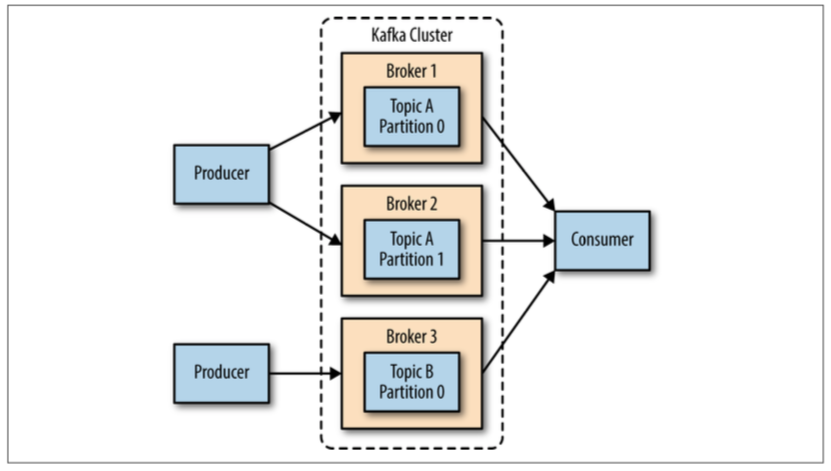
\includegraphics[width=0.90000\textwidth]{../images/kafka-cluster.png}
\caption{Esempio di cluster \label{figure_5}}
\end{figure}

A capo di un cluster troviamo un broker \emph{leader} al quale tutti gli
altri broker del cluster devono far riferimento per permette ai
meccanismi di replicazioni dei messaggi di funzionare correttamente: una
partizione può essere assegnata a più broker, questo permette al cluster
di poter gestire fallimenti dei brokers. In ogni cluster un particolare
broker viene eletto a \emph{controller}, ovvero un broker con l'incarico
di gestire la suddivisione delle partizioni sull'intero cluster e di
monitorare l'andamento del cluster.

\begin{figure}
\centering
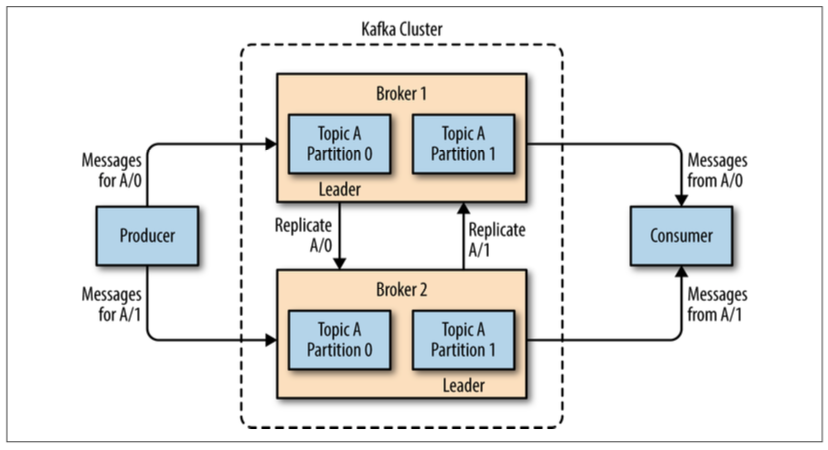
\includegraphics[width=0.90000\textwidth]{../images/partition-replica.png}
\caption{Gestione delle repliche \label{figure_5}}
\end{figure}

Una funzionalità importante di Kafka è la possibilità di utilizzare i
topic come database di messaggi persistenti.\\
I messaggi vengono tenuti in memoria per un particolare periodo di tempo
oppure in base allo spazio di memoria di occupato, entrambe le opzioni
sono configurabili alla creazione di un broker, vi è poi la possibilità
di abilitare la \emph{log compaction} ovvero un meccanismo che permette
a Kafka di mantenere in memoria \emph{solo gli ultimi messaggi
indicizzati su un indicativo specifico}.

\newpage

\subsubsection{5.7. Schema}\label{schema}

Nonostante i messaggi in Kafka non siano altro che degli array di byte è
fortemente consigliato l'uso di \emph{schema} per la gestione e l'uso
della struttura dei record.

Lo \emph{schema} è la struttura o organizzazione logicati dei dati
contenuti in un topic e nel caso specifico di Kafka, la scelta dei
formati disponibili ricade spesso su di un singolo formato: Apache Avro.
Esistono altre scelte possibili come Javascript Object Notation (JSON)
oppure Extensible Markup Language (XML), ma Avro offre una serie di
vantaggi rispetto a questo genere di schemi oltre ad avere alcune
implementazioni ad-hoc in Kafka. Avro è diventato nel tempo lo standard
per gli schema nelle applicazioni basate su Kafka, gli stessi
sviluppatori di Kafka ne promuovono l'uso citando una serie di motivi:

\begin{itemize}
\tightlist
\item
  Avro è mappabile su JSON
\item
  Al contrario di JSON, è possibile scomporre lo schema dei dati dalla
  definizione dell'oggetto
\item
  E' un linguaggio maturo ben supportato dalla community; Esistono molte
  librerie che permettono di creare automaticamente oggetti Java o case
  classes in Scala partendo da uno schema Avro
\end{itemize}

Apache Avro è un formato per la serializzazione di dati, ogni messaggio
Avro si divide in due parti: i \emph{dati} e lo \emph{schema dei dati}.

Un esempio di \textbf{schema dei dati} di un record con cinque campi:
\small

\begin{Shaded}
\begin{Highlighting}[]
\FunctionTok{\{}
  \DataTypeTok{"type"}\FunctionTok{:} \StringTok{"record"}\FunctionTok{,}
  \DataTypeTok{"doc"}\FunctionTok{:}\StringTok{"This event records the sale of a product"}\FunctionTok{,}
  \DataTypeTok{"name"}\FunctionTok{:} \StringTok{"ProductSaleEvent"}\FunctionTok{,}
  \DataTypeTok{"fields"} \FunctionTok{:} \OtherTok{[}
    \FunctionTok{\{}\DataTypeTok{"name"}\FunctionTok{:}\StringTok{"time"}\FunctionTok{,} \DataTypeTok{"type"}\FunctionTok{:}\StringTok{"long"}\FunctionTok{,} \DataTypeTok{"doc"}\FunctionTok{:}\StringTok{"The time of the purchase"}\FunctionTok{\}}\OtherTok{,}
    \FunctionTok{\{}\DataTypeTok{"name"}\FunctionTok{:}\StringTok{"customer_id"}\FunctionTok{,} \DataTypeTok{"type"}\FunctionTok{:}\StringTok{"long"}\FunctionTok{,} \DataTypeTok{"doc"}\FunctionTok{:}\StringTok{"The customer"}\FunctionTok{\}}\OtherTok{,}
    \FunctionTok{\{}\DataTypeTok{"name"}\FunctionTok{:}\StringTok{"product_id"}\FunctionTok{,} \DataTypeTok{"type"}\FunctionTok{:}\StringTok{"long"}\FunctionTok{,} \DataTypeTok{"doc"}\FunctionTok{:}\StringTok{"The product"}\FunctionTok{\}}\OtherTok{,}
    \FunctionTok{\{}\DataTypeTok{"name"}\FunctionTok{:}\StringTok{"quantity"}\FunctionTok{,} \DataTypeTok{"type"}\FunctionTok{:}\StringTok{"int"}\FunctionTok{\}}\OtherTok{,}
    \FunctionTok{\{}\DataTypeTok{"name"}\FunctionTok{:}\StringTok{"payment"}\FunctionTok{,}
        \DataTypeTok{"type"}\FunctionTok{:\{}\DataTypeTok{"type"}\FunctionTok{:}\StringTok{"enum"}\FunctionTok{,}
            \DataTypeTok{"name"}\FunctionTok{:}\StringTok{"payment_types"}\FunctionTok{,}
                \DataTypeTok{"symbols"}\FunctionTok{:}\OtherTok{[}\StringTok{"cash"}\OtherTok{,}\StringTok{"mastercard"}\OtherTok{,}\StringTok{"visa"}\OtherTok{]}\FunctionTok{\},}
        \DataTypeTok{"doc"}\FunctionTok{:}\StringTok{"The method of payment"}\FunctionTok{\}}
  \OtherTok{]}
\FunctionTok{\}}
\end{Highlighting}
\end{Shaded}

\normalsize
\newpage
Ed un generico record di \textbf{dati} definito in base allo schema:

\small

\begin{Shaded}
\begin{Highlighting}[]
\FunctionTok{\{}  
  \DataTypeTok{"time"}\FunctionTok{:} \DecValTok{1424849130111}\FunctionTok{,}     
  \DataTypeTok{"customer_id"}\FunctionTok{:} \DecValTok{1234}\FunctionTok{,}  
  \DataTypeTok{"product_id"}\FunctionTok{:} \DecValTok{5678}\FunctionTok{,}  
  \DataTypeTok{"quantity"}\FunctionTok{:} \DecValTok{3}\FunctionTok{,}  
  \DataTypeTok{"payment_type"}\FunctionTok{:} \StringTok{"mastercard"}  
\FunctionTok{\}}
\end{Highlighting}
\end{Shaded}

\normalsize

In Kafka ogni topic posside un particolare schema Avro im modo da :

\begin{itemize}
\tightlist
\item
  definire la struttura dei messaggi pubblicabili nel topic
\item
  permettere a producers e consumers di conoscere quali sono i campi dei
  messaggi del topic e qual'è il loro tipo
\item
  documentare la tipologia dei messaggi pubblicati nel topic
\item
  evitare la presenza di dati corrotti nel topic
\end{itemize}

Questo genere di meccanismo per la gestione dei dati diventa di assoluta
importanza all'aumentare delle applicazioni che dipendono dall'utilizzo
dei dati prodotti e gestiti da una piattaforma Kafka, evitando problemi
``effetto Domino'' dove un singolo errore in un messaggio potrebbe
portare a corrompere un consumer o applicazioni terze che utilizzano i
dati forniti dal consumer.

Un formato dei dati consistente come Avro permette di \emph{disacoppiare
i formati utilizzati per la lettura e la scrittura dei messaggi}, ovvero
viene data la possibilità alle applicazioni che si iscrivono ad un
particolare topic di poter utilizzare un nuovo schema di dati
compatibile con un vecchio formato, senza dover aggiornare tutte le
applicazioni che utilizzano ancora il vecchio formato.

Supponiamo ad esempio di utilizzare un formato del tipo seguente per
gestire le informazioni riguardando agli acquirenti di un particolare
servizio/piattaforma:

\small 

\begin{Shaded}
\begin{Highlighting}[]
\FunctionTok{\{}
    \DataTypeTok{"namespace"}\FunctionTok{:} \StringTok{"customerManagement.avro"}\FunctionTok{,}
    \DataTypeTok{"type"}\FunctionTok{:} \StringTok{"record"}\FunctionTok{,}
    \DataTypeTok{"name"}\FunctionTok{:} \StringTok{"Customer"}\FunctionTok{,}
    \DataTypeTok{"fields"}\FunctionTok{:} \OtherTok{[}
         \FunctionTok{\{}\DataTypeTok{"name"}\FunctionTok{:} \StringTok{"id"}\FunctionTok{,} \DataTypeTok{"type"}\FunctionTok{:} \StringTok{"int"}\FunctionTok{\}}\OtherTok{,}
         \FunctionTok{\{}\DataTypeTok{"name"}\FunctionTok{:} \StringTok{"name"}\FunctionTok{,}  \DataTypeTok{"type"}\FunctionTok{:} \StringTok{"string"}\FunctionTok{\}}\OtherTok{,}
         \FunctionTok{\{}\DataTypeTok{"name"}\FunctionTok{:} \StringTok{"faxNumber"}\FunctionTok{,} \DataTypeTok{"type"}\FunctionTok{:} \OtherTok{[}\StringTok{"null"}\OtherTok{,} \StringTok{"string"}\OtherTok{]}\FunctionTok{,} \DataTypeTok{"default"}\FunctionTok{:} \StringTok{"null"}\FunctionTok{\}}
    \OtherTok{]} 
\FunctionTok{\}}
\end{Highlighting}
\end{Shaded}

\normalsize

Una applicazione che vuole utilizzare lo stream di dati di questo topic
avrà probabilmente dei metodi come \texttt{getId()}, \texttt{getName()}
e \texttt{getFaxNumber()} per leggere i dati del topic; Di nota è il
tipo del campo \texttt{faxNumber} il quale è esplicitamente possibile
che sia \texttt{null}, ovvero è lecito aspettarsi che l'applicazione che
utilizza questi dati non si romperà nel caso in cui il fax non sia
presente nel messaggio.

Supponiamo di aver utilizzato lo schema precedente per genere una
importante mole di dati in un topic ma di voler migrare il nostro schema
ad un nuovo formato che permetta agli utenti di specificare la loro
\texttt{email} piuttosto che il loro fax.

\small

\begin{Shaded}
\begin{Highlighting}[]
\FunctionTok{\{}
    \DataTypeTok{"namespace"}\FunctionTok{:} \StringTok{"customerManagement.avro"}\FunctionTok{,}
    \DataTypeTok{"type"}\FunctionTok{:} \StringTok{"record"}\FunctionTok{,}
    \DataTypeTok{"name"}\FunctionTok{:} \StringTok{"Customer"}\FunctionTok{,}
    \DataTypeTok{"fields"}\FunctionTok{:} \OtherTok{[}
         \FunctionTok{\{}\DataTypeTok{"name"}\FunctionTok{:} \StringTok{"id"}\FunctionTok{,} \DataTypeTok{"type"}\FunctionTok{:} \StringTok{"int"}\FunctionTok{\}}\OtherTok{,}
         \FunctionTok{\{}\DataTypeTok{"name"}\FunctionTok{:} \StringTok{"name"}\FunctionTok{,}  \DataTypeTok{"type"}\FunctionTok{:} \StringTok{"string"}\FunctionTok{\}}\OtherTok{,}
         \FunctionTok{\{}\DataTypeTok{"name"}\FunctionTok{:} \StringTok{"email"}\FunctionTok{,} \DataTypeTok{"type"}\FunctionTok{:} \OtherTok{[}\StringTok{"null"}\OtherTok{,} \StringTok{"string"}\OtherTok{]}\FunctionTok{,} \DataTypeTok{"default"}\FunctionTok{:} \StringTok{"null"}\FunctionTok{\}}
    \OtherTok{]} 
\FunctionTok{\}}
\end{Highlighting}
\end{Shaded}

\normalsize

Ancora una volta l'applicazione che utilizza questo schema avrà dei
metodi \texttt{getId()}, \texttt{getName()} ma invece di
\texttt{getFaxNumber()} avrà \texttt{getEmail()}; Dopo l'aggiornamento
dello schema, i vecchi messaggi presenti nel topic conterranno il campo
\texttt{faxNumber} mentre i nuovi messaggi avranno il campo
\texttt{email}.

Dato che il tipo dei campi \texttt{faxNumber} e \texttt{email} può
essere sia \texttt{string} che \texttt{null}, nessuna delle tue
tipologie di applicazioni potrà fallire: la vecchia tipologia di
applicazioni semplicemente registrerà i nuovi messaggi come utenti senza
un numero di fax, mentre le nuove applicazioni vedranno i vecchi
messaggi del topic come utenti senza una email.

Questo genere di \emph{evoluzione} dello schema dei dati di un topic è
il motivo centrale dietro all'uso della tecnologia: garantire la
robustezza dei dati senza compromettere la leggibilità dello schema o il
funzionamento di applicazioni che utilizzano lo stesso topic.\\
L'evoluzione dello schema è permessa solo secondo determinate regole di
compatibilità la cui definizione esula dal contesto di questo tesi ma
che possono essere visionate nella
\href{https://avro.apache.org/docs/1.7.7/spec.html\#Schema+Resolution}{documentazione
di Apache Avro}.

\newpage

\subsubsection{5.8. Schema Registry}\label{schema-registry}

Uno dei vantaggi di Avro rispetto a JSON è la possibilità di non dover
inserire lo schema dei dati ``completo'' in ogni record permettendo di
pubblicare su un topic dei messaggi meno pesanti ed è proprio per
sfruttare questo vantaggio che nasce lo \emph{Schema Registry}.\\
Uno \emph{schema registry} è un servizio di gestione degli schema Avro
utilizzato da Kafka per servire ed evolvere i metadati di un topic; E'
utilizzato dai producers nella fase di scrittura (serializzazione di un
messaggio), dai consumer nella fase di lettura (deserializzazione di un
messaggio) ed impone delle regole di forma a tutti i client che
intendono utilizzare un topic specificato con formato dati Avro.

\begin{figure}
\centering
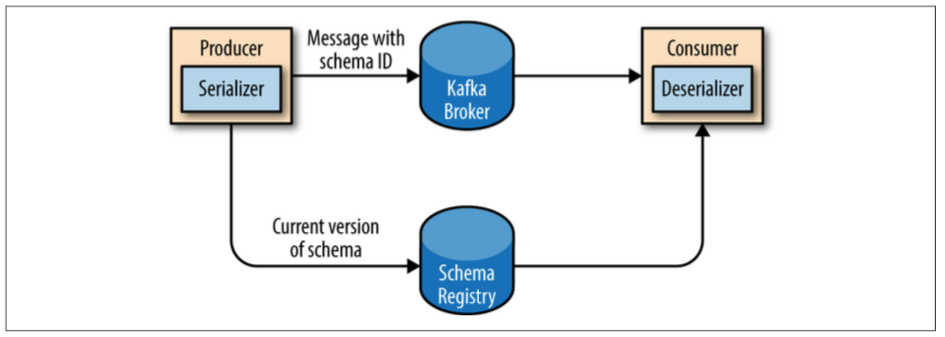
\includegraphics[width=0.90000\textwidth]{../images/schema-registry.png}
\caption{Serializzazione e deserializzazione con schema registry
\label{figure_5}}
\end{figure}

Supponiamo di avere uno schema registry e di voler produrre dei messaggi
su di un topic:

\begin{enumerate}
\def\labelenumi{\arabic{enumi}.}
\tightlist
\item
  Il producer interrogherà il registry per sapere se esiste già uno
  schema dei dati per un particolare topic inviando la propria copia
  dello schema, in caso contrario sarà lui stesso a pubblicarlo nel
  registry.
\item
  Lo schema registry verifica se lo schema ricevuto dal producer è
  uguale o una evoluzione compatibile dello schema già presente, in caso
  negativo verrà alzata un eccezzione e vietata la scrittura al
  producer.
\item
  Se lo schema proposto dal producer è valido, nel record Avro verrà
  inserito un riferimento allo schema del topic.
\end{enumerate}

L'utilizzo dello schema registry da parte di un consumer è speculare a
quello di un producer.

\newpage

\subsection{6. Architetture
Event-driven}\label{architetture-event-driven}

\subsubsection{6.1. Kafka come piattaforma per Event
Sourcing}\label{kafka-come-piattaforma-per-event-sourcing}

Il pattern Event Sourcing e la piattaforma Apache Kafka sono accomunati
da uno specifico elemento: \emph{il log}.

Entrambe le soluzioni utilizzano la medesima struttura dati per
risolvere un particolare problema, è quindi spontaneo che nel tempo ES
sia diventato un pattern predominante nelle applicazioni dell'ecosistema
Kafka.

Riassumendo i capitoli precedenti, Event Sourcing utilizza il log come
struttura dati per poter mantenere una sequenza immutabile di eventi
generati da una applicazione o da più parti di un sistema; Questa
sequenza di eventi definisce la storia del sistema e può essere
utilizzato per ricavare lo stato del sistema in un qualsiasi momento
della sua vita.

\begin{figure}
\centering
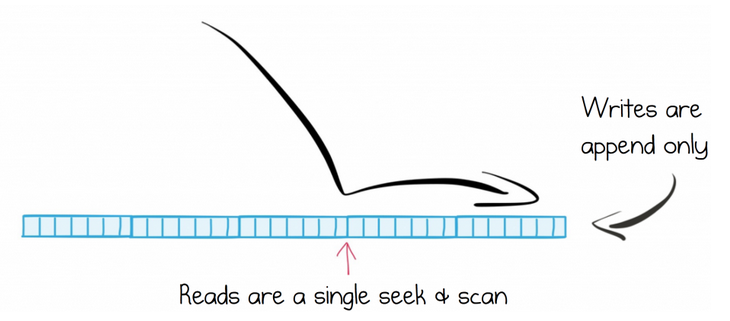
\includegraphics[width=0.80000\textwidth]{../images/log-kafka.png}
\caption{Scrittura e lettura da un log \label{figure_5}}
\end{figure}

Il log è una struttura dati fondamentale e naturalmente efficiente dato
il caso d'uso: sia la lettura che la scrittura di dati da un log (o
topic Kafka) sono sequenziali e sfruttano a pieno le funzionalità di
batching e caching offerte da Kafka.

Nel caso di un producer, l'operazione di inserimento di un nuovo
elemento nel topic è estremamente efficiente in quanto si tratta di un
semplice inserimento in coda di costo \(O(1)\), e nel caso di utilizzo
di un consumer la lettura da un topic sarà sempre effettuata in batch e
sequenziale (che sia dall'inizio del topic o da un particolare offset è
irrilevante) e quindi anche in questo caso avrà costo \(O(1)\).\\
Il limite imposto dalla lettura sequenziale di un topic permette inoltre
una riduzione dei costi di gestione della piattaforma non dovendo
gestire in memoria indici tipici di altre strutture dati come tabelle
hash o alberi, utilizzati per letture indicizzate o cancellazioni.

La lettura sequenziale di un topic è pur sempre un limite della
piattaforma ma che nel caso d'uso di una applicazione sviluppata
seguendo event sourcing diventa assolutamente irrilevante in quanto è lo
stesso pattern a premere per l'utilizzo di un log come event store.

L'utilizzo di Kafka come Event Store è un altro dei motivi che rende la
piattaforma un ottimo strumento da utilizzare con Event Sourcing.\\
Perchè una piattaforma possa funzionare come database/event store è
necessario che sia \emph{affidabile}, \emph{modulare} e dotata di
strumenti per la creazione di \emph{viste} degli eventi registrati.

Kafka è \emph{modulare} grazie al sistema dei brokers, il quale permette
uno svilippo dei consumer orizzontale, performante ed ``elastico'',
facilmente ridimensionabile a seconda della mole di dati presente nel
sistema.

Kafka è inoltre \emph{affidabile} su più fronti:

\begin{itemize}
\tightlist
\item
  nonostante non sia una qualità necessariamente utile in un sistema che
  utilizza ES, la \emph{temporabilità} dei messaggi è garantita
  attraverso la definizione di una chiave al momento della pubblicazione
  dei messaggi oppure tramite l'utilizzo di una singola partizione.
\item
  la \emph{durabilità} dei messaggi è garantita dal meccanismo di
  replica su più partizioni.
\item
  l'utilizzo dello schema registry garantisce maggiore sicurezza nel
  caso di \emph{evoluzione dello schema dei dati}, rendendo disponibile
  uno strumento che automaticamente valida nuove evoluzione della forma
  dei dati aiutando gli sviluppatori nel creare soluzioni
  ``backward-compatible''.
\item
  il log, con la sua qualità di \emph{immutabilità}, oltre ad essere la
  struttura dati dominante della piattaforma ne è anche il \emph{sistema
  di versioning dei dati}, garantendo l'esistenza di una
  \emph{cronologia non modificabile} di tutti gli eventi che sono stati
  registrati.
\item
  la possibilità di creare un numero arbitrario di topic permette la
  \emph{segmentazione} dei dati/eventi secondo la granularità che il
  team di sviluppo ritiene più opportuna; Non è assolutamente sbagliato
  sviluppare una soluzione con microservizi che utilizzato topic
  `privati' per le loro necessità e topic `publici' per comunicare tra
  loro.
\end{itemize}

\begin{figure}
\centering
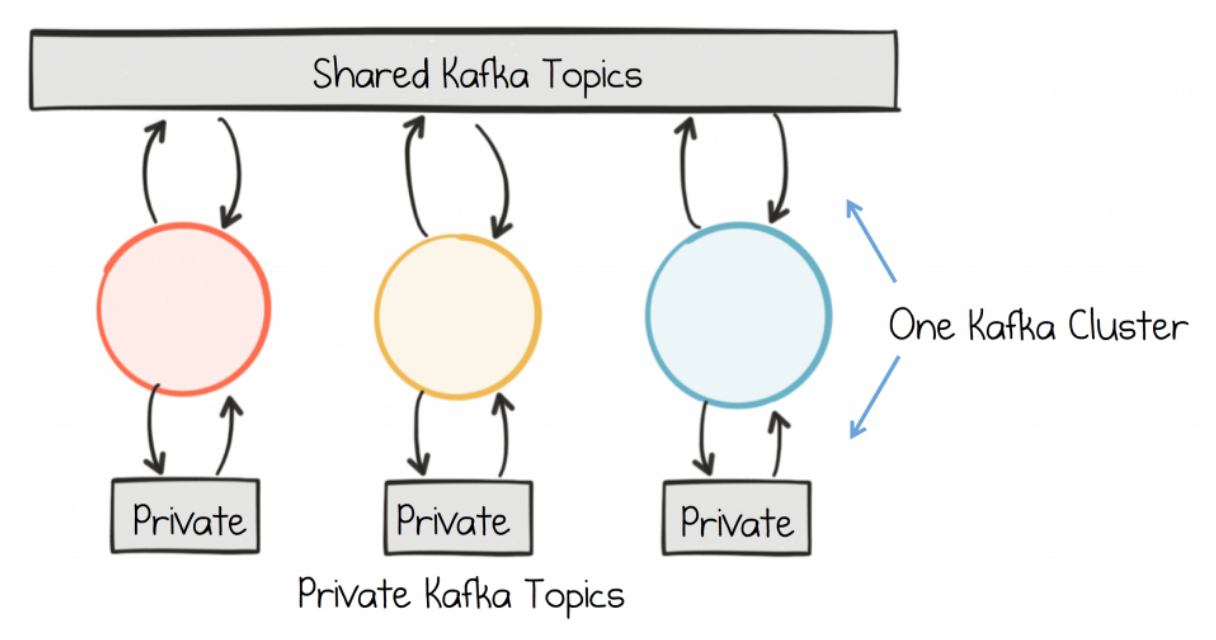
\includegraphics[width=0.70000\textwidth]{../images/public-private-topics.png}
\caption{Topic publici e privati in un sistema distribuito
\label{figure_5}}
\end{figure}

\begin{itemize}
\tightlist
\item
  Kafka permette di specificare per quanto tempo mantenere l'intero
  stato dei propri topic, rendendo di fatto la piattaforma un ``database
  per eventi''.
\item
  attraverso l'uso di \emph{Kafka Connect API} è estremamente facile
  leggere e scrivere dati da/a database \emph{esterni}.
\item
  per la lettura e pubblicazione di dati da/a Kafka a microservizi
  \emph{Kafka Streams API} offre una soluzione semplice e ad-hoc basata
  su event store.
\end{itemize}

Il pattern event sourcing si basa sull'idea di avere una sequenza di
eventi che, ove necessario, è possibile eseguire per ottenere lo stato
corrente del sistema; In genere la costruzione dello stato attuale della
piattaforma è una operazione dispendiosa e ES non dovrebbe essere preso
in considerazione se l'unico approccio all'analisi o uso dei dati del
sistema è una serie di query allo stato attuale, ma è anche vero che
avere una vista aggiornata dello stato corrente può essere utile anche
per quei sistemi che decidono di abbracciare completamente l'approccio
basato sugli eventi.

I topic in Kafka sono dei log di eventi immutabili ma con una
particolarità: è possibile \emph{comprimerli} in base al valore della
chiave.

\begin{figure}
\centering
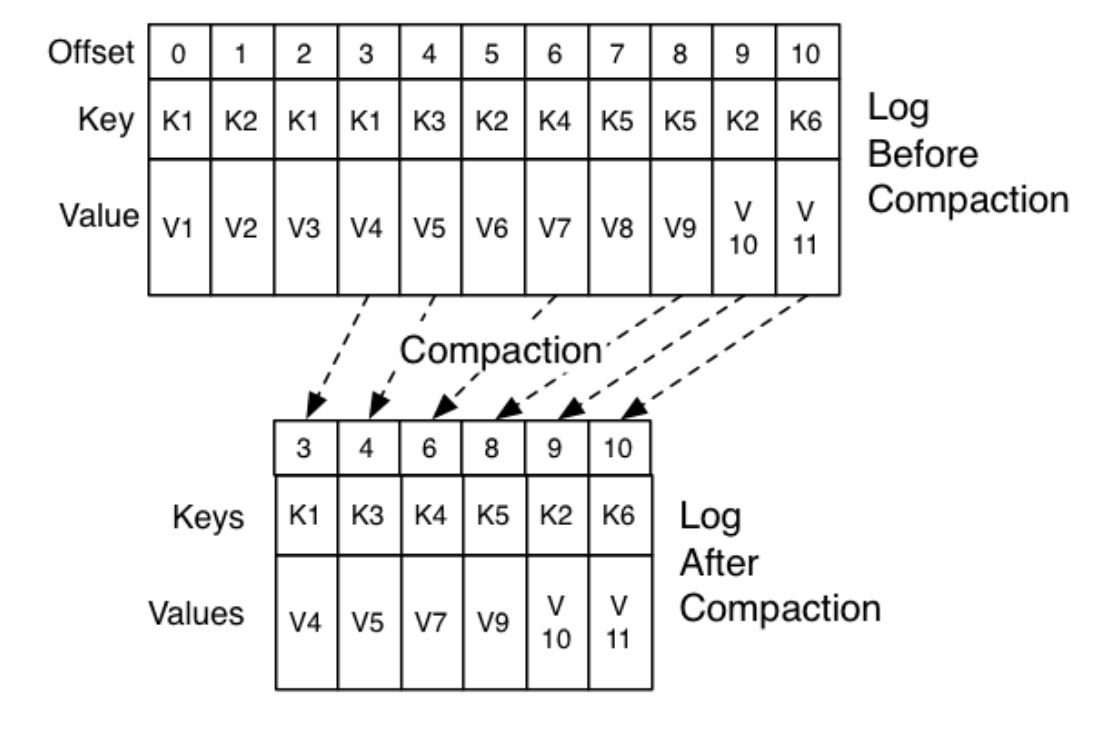
\includegraphics[width=0.80000\textwidth]{../images/log-compaction.png}
\caption{Log compaction \label{figure_5}}
\end{figure}

Il sistema di \emph{log compaction} garantisce che Kafka, dato un topic,
conserverà solamente l'ultimo messaggio a parità di chiave pubblicato
sullo stesso topic.\\
Questa funzionalità può quindi essere utilizzata come \emph{vista dello
stato corrente del sistema} o di alcune sue parti oppure come
\emph{meccanismo di difesa} per la fase di recovery post-crash del
sistema.

Il problema del calcolo del stato corrente è quindi risolto affiancando
ai log utilizzati come stream di eventi un topic compresso ``istanza''
del stato del sistema.

E' da notare che questo meccanismo di compressione dei log può anche
essere utilizzato per archiviare parte di un vecchio log in modo da
risparmiare spazio in memoria.

\subsection{6.2. Kafka Connect: sistemi legacy, database ed Event
Sourcing}\label{kafka-connect-sistemi-legacy-database-ed-event-sourcing}

Se si decide di sviluppare un nuovo progetto partendo da zero ed
utilizzando Kafka ed ES, non è difficile immaginare che creare la nuova
struttura sarà relativamente semplice in quanto ci ritroveremo a
sviluppare soluzioni software basate su eventi e verrà naturale
pubblicare questi eventi su Kafka.\\
Nel caso in cui si decida di addottare Kafka ed ES su un vecchio
progetto sorgono spontanee domande come ``Quali sono i miei eventi?'',
``Come posso utilizzare i database già presenti?'' oppure ``Ultimata la
migrazione che fine faranno i vecchi database e le vecchie
applicazioni?''. Domande come queste sono risolte dalla \emph{Connect
API} di Kafka.

Kafka Connect è un framework che permette di integrare Kafka con
moltissime delle soluzioni database già presenti sul mercato (MySQL,
PostgreSQL, Elasticearch, Mongo, ecc.).\\
Il framework si basa sull'uso di \emph{Source connectors} per importare
dati da sorgenti esterne e \emph{Sink connectors} per la fase di
scrittura su strutture esterne; Kafka viene rilasciato di base con molti
connettori già pronti e testati all'uso e molti altri sviluppati dalla
community open-source sono disponibili online. E' inoltre prevista la
possibilità di sviluppare connettori custom per soluzioni più
particolari del normale.

I source connector funzionano facendo leva sul log transazionale
generato con tramite Change Data Capture (CDC) del database sorgente,
che non è altro che un log sul quale vengono scritte, in ordine
temporale, tutte le operazioni di insert, update e delete fatte sul
database in questione. E' facile immaginare che questo log transazionale
è facilmente utilizzabile per definire lo stream di eventi necessario a
Kafka per funzionare, ed è esattamente cosi che funzionano i connettori:
definita una configurazione per il connettore, il transactional log del
database viene copiato su di un topic Kafka.\\
Esistono ovviamente delle differenze nel funzionamento di alcuni
connettori (alcuni database supportano CDC basato su polling, altri su
meccanismi push-pull, ecc.) ma il risultato del procedimento di
creazione del topic legato al database sorgente sarà sempre lo stesso.\\
Specularmente i sink connector sono invece utilizzati per operazioni di
write/update su dei database partendo da un topic specificato.\\
Di nota è la possibilità, grazie ai sink connectors, di utilizzare
svariati database come data store per topic compressi, garatendo cosi al
sistema la possibilità di sfruttare le classiche tecnologie basate su
database per tutte quelle operazioni di query dei dati per il quale
Kafka non è necessariamente la soluzione migliore.

\newpage

Utilizzando source e sink connectors è quindi possibile creare pipeline
complesse di dati tra Kafka, vari database e architetture ``legacy'' in
modo da permettere al sistema di evolversi gradualmente verso una
soluzione basata solamente su Kafka (se necessario).\\
Si immagini ad esempio di utilizzare i vecchi dati presenti in una
applicazione legacy per popolare i topic della piattaforma Kafka e
parallelamente sviluppare nuove soluzioni basata sulla nuova
architettura per raggiungere gli utenti della applicazione.

\begin{figure}
\centering
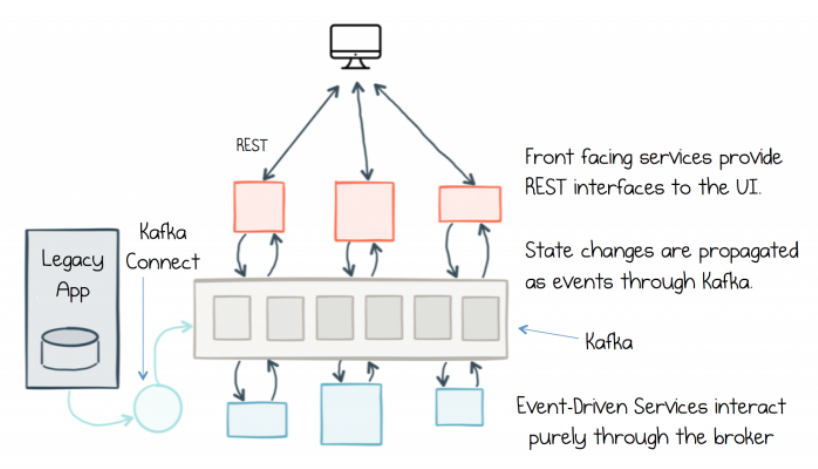
\includegraphics[width=1.05000\textwidth]{../images/legacy-kafka.png}
\caption{Architettura legacy con servizi Kafka \label{figure_5}}
\end{figure}

Un esempio potrebbe essere quello di un e-commerce: potremmo immaginare
di avere il servizio di gestione e creazione dell'inventario come la
nostra ``legacy app'' nell'immagine, mentre potremmo avere il servizio
di validazione dell'ordine (conferma dell'ordine, informazioni di
tracking, ecc.) gestito tramite Kafka.

\newpage

\subsection{6.3. Kafka Streams}\label{kafka-streams}

Per poter sviluppare soluzioni software basate sullo stream di eventi di
topic è necessario trovare una soluzione per poter avere accesso a
questi dati da un qualsiasi linguaggio di programmazione; Questa
soluzione è data dalla libreria \emph{Kafka Streams}.\\
Kafka Streams è una libreria che fornisce una astrazione sul concetto di
state store proposto da Kafka in modo da creare applicazioni o
microservizi con uno qualsiasi dei linguaggi supportati (Java o
Scala).\\
Uno state store è un database chiave-valore creato per interfacciarsi
con un topic Kafka, è possibile leggere e scrivere da un topic Kafka
semplicemente utilizzando le funzioni proposte dalla libreria.\\
La libreria offre delle primitive per creare delle applicazioni basato
sul concetto di \emph{topologie}, ovvero un grafo di stream processors
(i nodi del grafo) connessi tra loro da stream di dati (i lati del
grafo.)

\begin{figure}
\centering
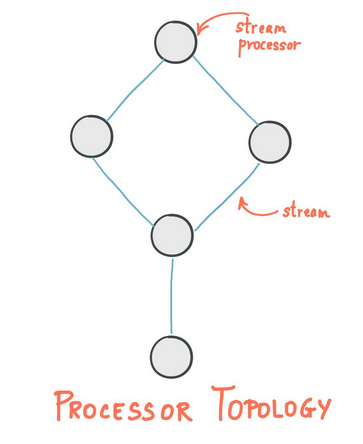
\includegraphics[width=0.50000\textwidth]{../images/topology-stream.png}
\caption{Generica topologia di una applicazione Kafka Stream
\label{figure_5}}
\end{figure}

Uno \emph{stream processor} è un nodo della topologia con il compito di
processare in qualche modo i dati che riceve. Ogni processor riceve dal
nodo precedente nella topologia un record alla volta, applica una
operazione al record e produce uno o più record in output verso tutti i
suoi successori.

Le operazioni eseguite da ogni nodo possono essere espremesse
utilizzando una Domain-specific Language (DSL) dichiarativa e funzionale
(esempi tipici sono funzioni come \texttt{map} e \texttt{filter}) oppure
una API di basso livello più vicina allo state store (e quindi più
lontana dall'astrazione utilizzata con la DSL).

Un esempio di un stream application che utilizza la stream DSL è dato
dal seguente codice Scala:

\small 

\begin{Shaded}
\begin{Highlighting}[]
\KeywordTok{package}\NormalTok{ io.}\FunctionTok{confluent}\NormalTok{.}\FunctionTok{examples}\NormalTok{.}\FunctionTok{streams}

\KeywordTok{import}\NormalTok{ java.}\FunctionTok{util}\NormalTok{.}\FunctionTok{Properties}

\KeywordTok{import}\NormalTok{ org.}\FunctionTok{apache}\NormalTok{.}\FunctionTok{kafka}\NormalTok{.}\FunctionTok{common}\NormalTok{.}\FunctionTok{serialization}\NormalTok{._}
\KeywordTok{import}\NormalTok{ org.}\FunctionTok{apache}\NormalTok{.}\FunctionTok{kafka}\NormalTok{.}\FunctionTok{streams}\NormalTok{._}
\KeywordTok{import}\NormalTok{ org.}\FunctionTok{apache}\NormalTok{.}\FunctionTok{kafka}\NormalTok{.}\FunctionTok{streams}\NormalTok{.}\FunctionTok{kstream}\NormalTok{.\{KStream, KStreamBuilder\}}

\KeywordTok{object}\NormalTok{ MapFunctionScalaExample \{}
  \KeywordTok{def} \FunctionTok{main}\NormalTok{(args: Array[String]) \{}
    \KeywordTok{val}\NormalTok{ builder = }\KeywordTok{new}\NormalTok{ KStreamBuilder}

    \KeywordTok{val}\NormalTok{ streamingConfig = \{}
      \KeywordTok{val}\NormalTok{ settings = }\KeywordTok{new}\NormalTok{ Properties()}
\NormalTok{      settings.}\FunctionTok{put}\NormalTok{(StreamsConfig.}\FunctionTok{BOOTSTRAP_SERVERS_CONFIG}\NormalTok{, }\StringTok{"localhost:9092"}\NormalTok{)}
\NormalTok{      settings.}\FunctionTok{put}\NormalTok{(StreamsConfig.}\FunctionTok{DEFAULT_KEY_SERDE_CLASS_CONFIG}\NormalTok{, }
\NormalTok{                    Serdes.}\FunctionTok{ByteArray}\NormalTok{.}\FunctionTok{getClass}\NormalTok{.}\FunctionTok{getName}\NormalTok{)}
\NormalTok{      settings.}\FunctionTok{put}\NormalTok{(StreamsConfig.}\FunctionTok{DEFAULT_VALUE_SERDE_CLASS_CONFIG}\NormalTok{, }
\NormalTok{                    Serdes.}\FunctionTok{String}\NormalTok{.}\FunctionTok{getClass}\NormalTok{.}\FunctionTok{getName}\NormalTok{)}
\NormalTok{      settings}
\NormalTok{    \}}

    \KeywordTok{val}\NormalTok{ text: KStream[Array[Byte], String] = builder.}\FunctionTok{stream}\NormalTok{(}\StringTok{"input-topic"}\NormalTok{)}
    \KeywordTok{val}\NormalTok{ upperCasedText: KStream[Array[Byte], String] = textLines.}\FunctionTok{mapValues}\NormalTok{(_.}\FunctionTok{toUpperCase}\NormalTok{())}
\NormalTok{    upperCasedText.}\FunctionTok{to}\NormalTok{(}\StringTok{"output-topic"}\NormalTok{)}
\NormalTok{  \}}
\NormalTok{\}}
\end{Highlighting}
\end{Shaded}

Nell'esempio, partendo dal topic \texttt{input-topic} viene creato uno
stream di record con chiave di tipo \texttt{ByteArray} e value (o
contenuto del messaggio) di tipo \texttt{String}.\\
Ad ogni messaggio viene applicata la funziona \texttt{.toUpperCase()}
tramite la funzione \texttt{.mapValues()} definita dalla DSL (e quindi
nodo della topologia di questa applicazione), infine viene pubblicato un
nuovo record con il nuovo messaggio (la stringa in maiuscolo) su un
nuovo topic \texttt{output-topic}.

\normalsize

\newpage

\hypertarget{conclusioni}{\subsection{7.
Conclusioni}\label{conclusioni}}

Nei capitoli precendenti ho presentato le idee alla base dell'utilizzo
di Apache Kafka, la sua architettura e il pattern (Event Sourcing) più
comunemente utilizzato per sviluppare soluzioni software con la
piattaforma; E' quindi ora necessario spiegare \emph{perchè} Apache
Kafka è una soluzione alternativa ai comuni processi di ETL e il
contesto che ha portato al suo sviluppo.

Nell'ultima decade la tipologia e mole di dati e i sistemi di analisi e
gestione di questi dati si sono trovati ad affrontare degli importanti
cambiamenti nell'ambito dei processi di ETL.\\
In passato si era abituati a sistemi di gestione/analisi dei dati
formati da più database operazionali che venivano utilizzati per creare
una pipeline di dati diretta verso una o più datawarehouse; Questo
processo di migrazione in genere non era richiesto che fosse eseguito
più di poche volte al giorno, ed è proprio questa scelta architetturale
che ha portato alla creazione dei vecchi tools di ETL.

\begin{figure}
\centering
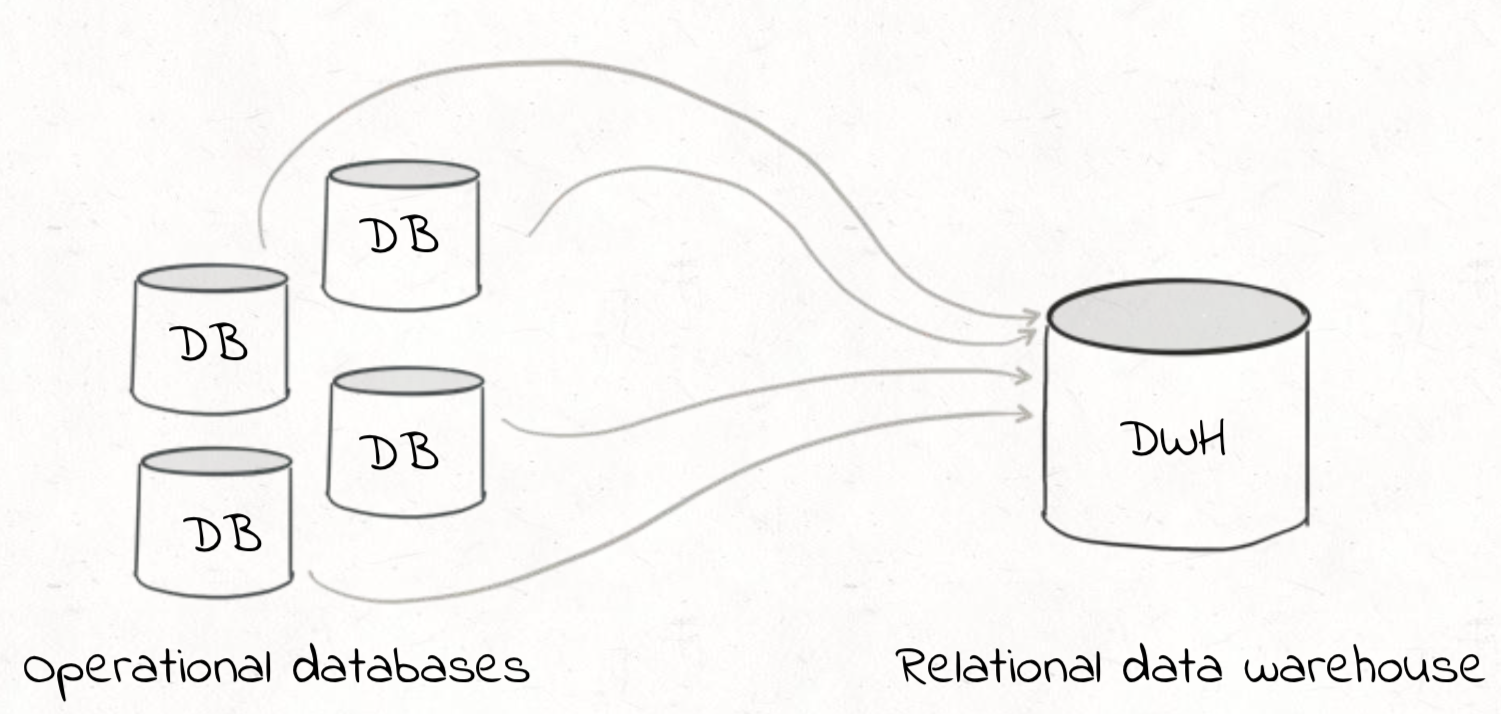
\includegraphics[width=0.90000\textwidth]{../images/op-dwh.png}
\caption{Database operazionali e datawarehouse \label{figure_5}}
\end{figure}

Lo scenario che si è presentanto negli ultimi anni è però completamente
diverso e può essere riassunto in pochi punti:

\begin{itemize}
\tightlist
\item
  Sempre più spesso, le vecchie architettura basate su un singolo
  database è scartata in favore di architetture formate da microservizi
  distribuiti che raccolgono dati da più fonti
\item
  Le tipologie di fonti di dati con cui interfaciarsi sono in rapida
  espansione, non esistono più solo database relazionali ma piuttosto,
  oltre agli stessi database relazionali, le aziende si trovano a dover
  fare uso di dati provienienti da database NoSQL, sensori, metriche e
  log delle tipologie più disparate e da un numero sempre crescente di
  sorgenti.
\item
  La spinta verso lo \emph{streaming} dei dati e una richiesta di
  aggiornamento dei dati ``istantanea'' porta il comune processo di ETL
  ad essere troppo lento per i moderni standard di analisi dei dati.
\end{itemize}

Questo non implica che un comune processo di ETL non può funzionare o
che non sia possibile sviluppare delle soluzioni ad-hoc a seconda dei
casi, il vero problema è che non avendo uno \emph{standard}, una
piattaforma o tecnologia con precise funzionalità atte a risolvere i
problemi di questo scenario spesso ci si ritrova davanti a sistemi
over-engineered o troppo complessi con capacità di sviluppo modulare
basse e difficilmente integrabili con nuove tecnologie emergenti.

Il risultato è che spesso una soluzione ad-hoc basato su un processo di
ETL finisce per essere un groviglio di pipeline tra applicazioni,
database e datawarehouse difficile da utilizzare e analizzare,
sopratutto in caso di emergenze.

\begin{figure}
\centering
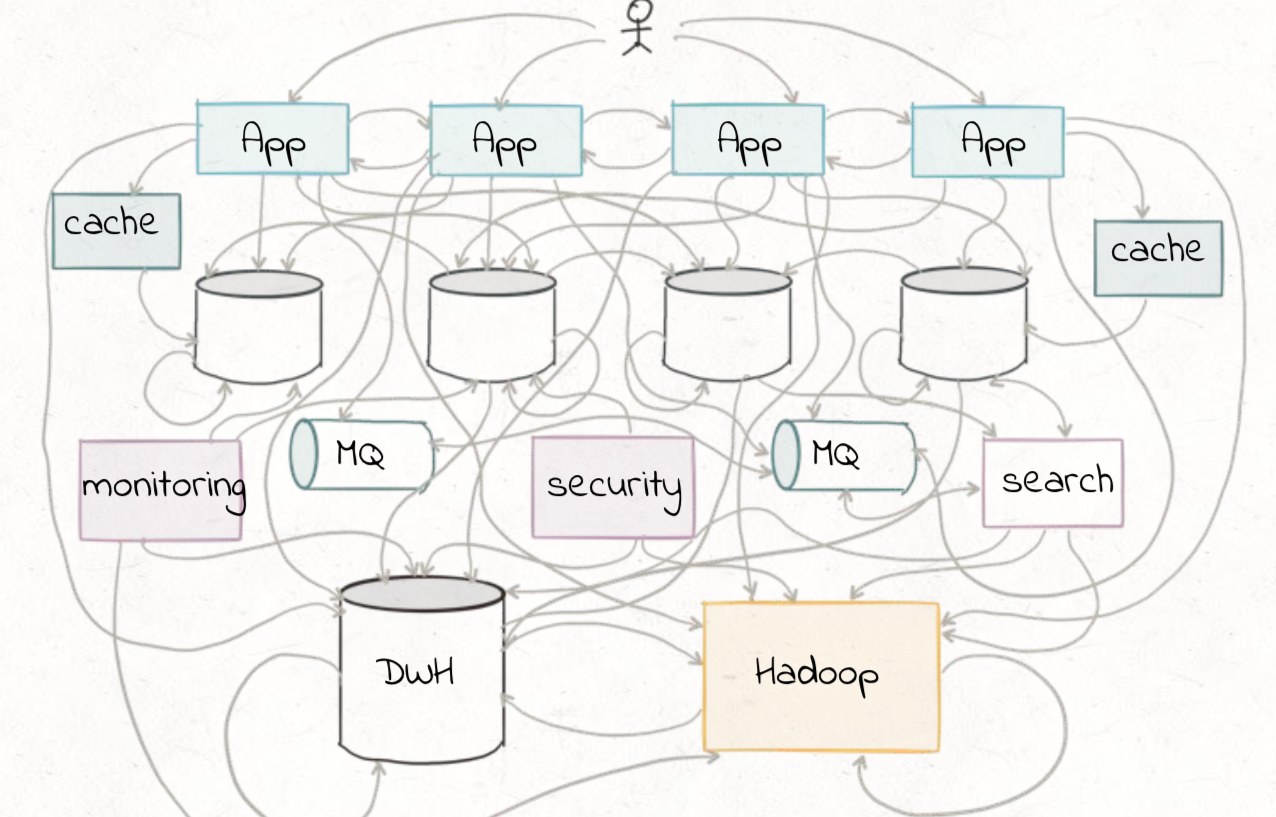
\includegraphics[width=0.90000\textwidth]{../images/etl-adhoc.png}
\caption{Soluzioni ETL ad-hoc \label{figure_5}}
\end{figure}

La necessità di sviluppare soluzioni ETL nasce durante gli anni '90, con
la montante richiesta da parte della grande distribuzione di poter
analizare le abitudini di acquisto online dei propri clienti.\\
In genere questo processo era formato da tre fasi, l'estrazione di dati
da più database operazionali, la trasformazione di questi dati in modo
che aderissero allo schema della data warehouse ed infine il caricamento
dei dati nella data warehouse. Con l'avanzare del tempo e della ricerca
in questo campo si è però giunti alla conclusione che la \emph{data
coverage} nelle datawarehouse è spesso molto bassa rispetto ai dati
presenti nei database operazionali, questo problema nasce dalla
difficoltà nel analizzare e trasformare moli di dati importanti
provenienti da più sorgenti (spesso con schemi di dati diversi) in
gruppi di dati omogeni rispetto allo schema delle data warehouse.

Lo scenario moderno ha essenzialmente bisogno di piattaforme di
real-time ETL, delle \emph{streaming platform}, capaci di processare
grossi volumi di dati delle tipologie più disparate, in tempo reale e
capaci di addattarsi a possibili sviluppi futuri nella propria
architettura (forward-compatible) come l'aggiunta di nuovi microservizi
o l'utilizzo di nuove sorgenti di dati.

\begin{figure}
\centering
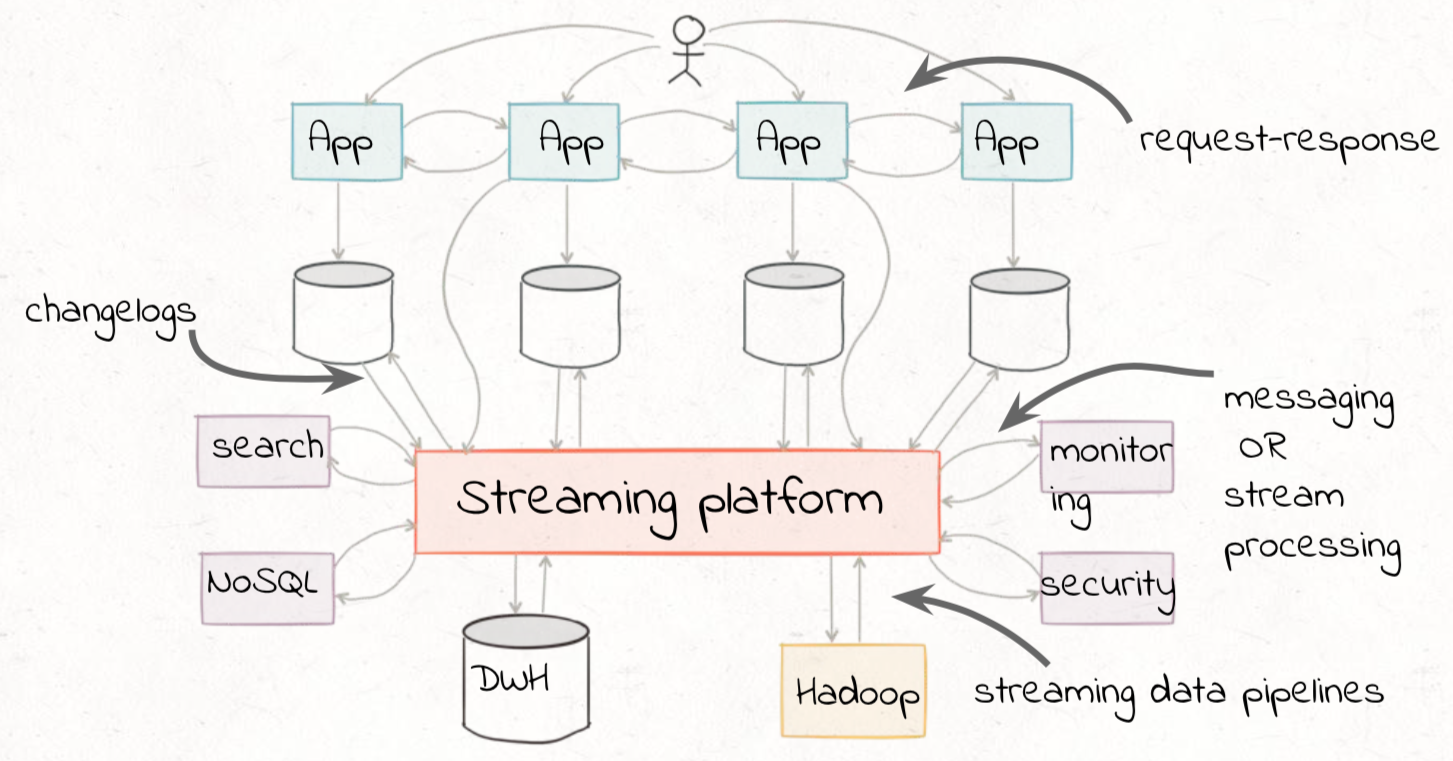
\includegraphics[width=0.90000\textwidth]{../images/streaming-platform.png}
\caption{Architettura basata su streaming platform \label{figure_5}}
\end{figure}

Sono esattamente queste necessità che hanno portato un gruppo di
sviluppatori di LinkedIn a sviluppare Apache Kafka, una streaming
platform ormai utilizzata da moltissime grandi aziende nel ambito dei
servizi web (Netflix, PayPal per citarne alcune). Kafka risolve tutti i
problemi presentati precedentemente:

\begin{itemize}
\tightlist
\item
  La necessità di gestire grossi volumi di dati in tempo reale è risolta
  grazie alla sua architettura basata sul concetto di log, l'utilizzo
  dei producers, consumers e lo schema registry presentati nei capitoli
  precedenti.
\item
  L'API Kafka Connect svolge il ruolo delle fasi di \emph{E}xtraction e
  \emph{L}oad dei processi di ETL, fornendo uno strumento capace di
  mettere in collegamento la piattaforma Kafka con una moltitudine di
  fonti di dati sia per la lettura che la scrittura delle
  trasformazioni.
\item
  Il ruolo della fase di \emph{T}ransform nei processi ETL è svolto
  dall'API Kafka Streams, la quale permette di sviluppare soluzioni
  software con il quale trattare e trasformare i dati pubblicati sulla
  piattaforma Kafka.
\end{itemize}

Apache Kafka è una tecnologia importante, in continua crescita e in
continua adozione da moltissime realtà internazionali nell'ambito IT,
non per questo non ha debolezze.\\
Proprio perchè è una nuova tecnologia in continua evoluzione, le
capacità di una azienda di adattare i propri sistemi all'utilizzo di
Kafka sono strettamente legate alle loro capacità di adozione e studio
di nuove tecnologie e soluzioni architetturali.

Nonostante le difficoltà tecnologiche, non ci sono però dubbi che i
processi di ETL stiano subendo una forte spinta evolutiva e che le
piattaforme di streaming come Kafka rappresentano una valida alternativa
ed il futuro dei processi di analisi e gestione di grossi volumi di
dati.

\newpage

\hypertarget{bibliografia}{\subsection{8.
Bibliografia}\label{bibliografia}}

\small
[1] Narkhede, N. and Shapira, G. and Palino, T. (2017), \emph{Kafka: The
Definitive Guide: Real-Time Data and Stream Processing at Scale},
O'Reilly Media Inc.

{[}2{]} Kleppmann, M. (2016), \emph{Making Sense of Stream Processing},
O'Reilly Media Inc.

\hypertarget{sitografia}{\subsection{9. Sitografia}\label{sitografia}}

\small
[1] Martin F., \emph{Event Sourcing},\\
https://martinfowler.com/eaaDev/EventSourcing.html

{[}2{]} Wikipedia contributors. (2018), \emph{Event store},\\
https://en.wikipedia.org/w/index.php?title=Event\_store\&oldid=824633488

{[}3{]} Narkhede, N. \emph{ETL Is Dead, Long Live Streams: Real-Time
Streams with Apache Kafka},\\
www.youtube.com/watch?v=I32hmY4diFY

{[}4{]} Kreps J. (2013), \emph{The Log: What every software engineer
should know about real-time data's unifying abstraction},\\
https://engineering.linkedin.com/distributed-systems/log-what-every-software-engineer-should-know-about-real-time-datas-unifying

{[}5{]} Kreps J. (2015), \emph{Putting Apache Kafka To Use: A Practical
Guide to Building a Streaming Platform},\\
https://www.confluent.io/blog/stream-data-platform-1/

{[}6{]} Stopford B. (2016), \emph{The Data Dichotomy: Rethinking the Way
We Treat Data and Services},\\
https://www.confluent.io/blog/data-dichotomy-rethinking-the-way-we-treat-data-and-services/

{[}7{]} Stopford B. (2017), \emph{Build Services on a Backbone of
Events},\\
https://www.confluent.io/blog/build-services-backbon5-events/

{[}8{]} Stopford B. (2017), \emph{Using Apache Kafka as a Scalable,
Event-Driven Backbone for Service Architectures},\\
https://www.confluent.io/blog/apache-kafka-for-service-architectures/

{[}9{]} Stopford B. (2017), \emph{Messaging as the Single Source of
Truth},\\
https://www.confluent.io/blog/messaging-single-source-truth/

{[}10{]} Stopford B. (2017), \emph{Building a Microservices Ecosystem
with Kafka Streams and KSQL},\\
https://www.confluent.io/blog/building-a-microservices-ecosystem-with-kafka-streams-and-ksql/3

\end{document}
